\section{Connections and vector fields}

\subsection{The function \texorpdfstring{\( T \)}{T}}

We will build up a map \( T \) out of \( \oo \) which is meant to be like the circle bundle of a tangent bundle. And so we will begin with the intrinsic data of the link at each point: taking the link of a vertex gives us a map from vertices to polygons.

\begin{mydef}
\( T_0\defeq\link:\oo_0\to\EMzo \) is given by:
\begin{align*}
\link(w) &= brgo & \link(r) &= wbyg \\
\link(y) &= bogr & \link(g) &= wryo \\
\link(b) &= woyr & \link(o) &= wgyb
\end{align*}
We chose these orderings for the vertices in the link, by visualizing standing at the given vertex as if it were the north pole, then looking south and enumerating the link in clockwise order, starting from \( w \) if possible, else \( b \).
\end{mydef}

\begin{figure}[htbp]
\centering
\begin{figure}[h]
\centering
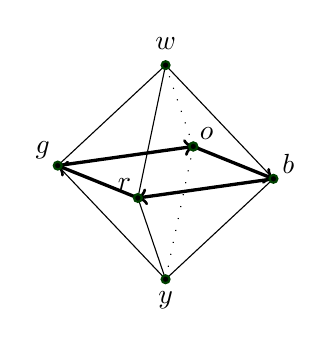
\begin{tikzpicture}%
  [x={(-0.860769cm, -0.121512cm)},
  y={(0.508996cm, -0.205391cm)},
  z={(-0.000053cm, 0.971107cm)},
  scale=1,
  eqback/.style={->, very thick},
  back/.style={loosely dotted, thin},
  eqedge/.style={->, very thick},
  edge/.style={black, thin},
  facet/.style={fill=blue!95!black,fill opacity=0.0},
  vertex/.style={inner sep=1pt,circle,draw=green!25!black,fill=black,thick}]
\coordinate (-1, -1, 0) at (-1, -1, 0);
\coordinate (-1, 1, 0) at (-1, 1, 0);
\coordinate (0, 0, -1) at (0, 0, -1);
\coordinate (0, 0, 1) at (0, 0, 1);
\coordinate (1, -1, 0) at (1, -1, 0);
\coordinate (1, 1, 0) at (1, 1, 0);
%% Drawing edges in the back
%%
\draw[edge,eqback] (-1, -1, 0) -- (-1, 1, 0);
\draw[edge,back] (-1, -1, 0) -- (0, 0, -1.4);
\draw[edge,back] (-1, -1, 0) -- (0, 0, 1.4);
\draw[edge,eqback] (1, -1, 0) -- (-1, -1, 0);
%% Drawing vertices in the back
%%
\node[vertex] at (-1, -1, 0)     {};
%% Drawing the facets
%%
\fill[facet] (1, 1, 0) -- (0, 0, -1.4) -- (1, -1, 0) -- cycle {};
\fill[facet] (1, 1, 0) -- (0, 0, 1.4) -- (1, -1, 0) -- cycle {};
\fill[facet] (1, 1, 0) -- (-1, 1, 0) -- (0, 0, 1.4) -- cycle {};
\fill[facet] (1, 1, 0) -- (-1, 1, 0) -- (0, 0, -1.4) -- cycle {};
%% Drawing edges in the front
%%
\draw[edge] (-1, 1, 0) -- (0, 0, -1.4);
\draw[edge] (-1, 1, 0) -- (0, 0, 1.4);
\draw[eqedge] (-1, 1, 0) -- (1, 1, 0);
\draw[edge] (0, 0, -1.4) -- (1, -1, 0);
\draw[edge] (0, 0, -1.4) -- (1, 1, 0);
\draw[edge] (0, 0, 1.4) -- (1, -1, 0);
\draw[edge] (0, 0, 1.4) -- (1, 1, 0);
\draw[eqedge] (1, 1, 0) -- (1, -1, 0);
%% Drawing the vertices in the front
%%
\begin{scope}[nodes=vertex]
\node[label=above right:\( b \)] at (-1, 1, 0)     {};
\node[label=below:\( y \)] at (0, 0, -1.4)     {};
\node[label=above:\( w \)] at (0, 0, 1.4)     {};
\node[label=above left:\( g \)] at (1, -1, 0)     {};
\node[label=above left:\( r \)] at (1, 1, 0)     {};
\node[label=above right:\( o \)] at (-1, -1, 0)     {};
\end{scope}
\end{tikzpicture}

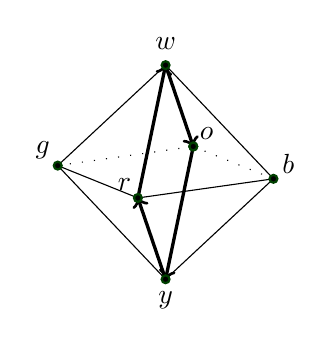
\begin{tikzpicture}%
  [x={(-0.860769cm, -0.121512cm)},
  y={(0.508996cm, -0.205391cm)},
  z={(-0.000053cm, 0.971107cm)},
  scale=1,
  eqback/.style={->, very thick},
  back/.style={loosely dotted, thin},
  eqedge/.style={->, very thick},
  edge/.style={black, thin},
  facet/.style={fill=blue!95!black,fill opacity=0.0},
  vertex/.style={inner sep=1pt,circle,draw=green!25!black,fill=black,thick}]
\coordinate (-1, -1, 0) at (-1, -1, 0);
\coordinate (-1, 1, 0) at (-1, 1, 0);
\coordinate (0, 0, -1) at (0, 0, -1);
\coordinate (0, 0, 1) at (0, 0, 1);
\coordinate (1, -1, 0) at (1, -1, 0);
\coordinate (1, 1, 0) at (1, 1, 0);
%% Drawing edges in the back
%%
\draw[edge,back] (-1, -1, 0) -- (-1, 1, 0);
\draw[edge,eqback] (-1, -1, 0) -- (0, 0, -1.4);
\draw[edge,eqback] (0, 0, 1.4) -- (-1, -1, 0);
\draw[edge,back] (1, -1, 0) -- (-1, -1, 0);
%% Drawing vertices in the back
%%
\node[vertex] at (-1, -1, 0)     {};
%% Drawing the facets
%%
\fill[facet] (1, 1, 0) -- (0, 0, -1.4) -- (1, -1, 0) -- cycle {};
\fill[facet] (1, 1, 0) -- (0, 0, 1.4) -- (1, -1, 0) -- cycle {};
\fill[facet] (1, 1, 0) -- (-1, 1, 0) -- (0, 0, 1.4) -- cycle {};
\fill[facet] (1, 1, 0) -- (-1, 1, 0) -- (0, 0, -1.4) -- cycle {};
%% Drawing edges in the front
%%
\draw[edge] (-1, 1, 0) -- (0, 0, -1.4);
\draw[edge] (-1, 1, 0) -- (0, 0, 1.4);
\draw[edge] (-1, 1, 0) -- (1, 1, 0);
\draw[edge] (0, 0, -1.4) -- (1, -1, 0);
\draw[eqedge] (0, 0, -1.4) -- (1, 1, 0);
\draw[edge] (0, 0, 1.4) -- (1, -1, 0);
\draw[eqedge] (1, 1, 0) -- (0, 0, 1.4) ;
\draw[edge] (1, 1, 0) -- (1, -1, 0);
%% Drawing the vertices in the front
%%
\begin{scope}[nodes=vertex]
\node[label=above right:\( b \)] at (-1, 1, 0)     {};
\node[label=below:\( y \)] at (0, 0, -1.4)     {};
\node[label=above:\( w \)] at (0, 0, 1.4)     {};
\node[label=above left:\( g \)] at (1, -1, 0)     {};
\node[label=above left:\( r \)] at (1, 1, 0)     {};
\node[label=above right:\( o \)] at (-1, -1, 0)     {};
\end{scope}
\end{tikzpicture}

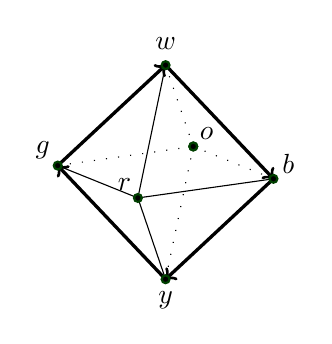
\begin{tikzpicture}%
  [x={(-0.860769cm, -0.121512cm)},
  y={(0.508996cm, -0.205391cm)},
  z={(-0.000053cm, 0.971107cm)},
  scale=1,
  eqback/.style={->, very thick},
  back/.style={loosely dotted, thin},
  eqedge/.style={->, very thick},
  edge/.style={black, thin},
  facet/.style={fill=blue!95!black,fill opacity=0.0},
  vertex/.style={inner sep=1pt,circle,draw=green!25!black,fill=black,thick}]
\coordinate (-1, -1, 0) at (-1, -1, 0);
\coordinate (-1, 1, 0) at (-1, 1, 0);
\coordinate (0, 0, -1) at (0, 0, -1);
\coordinate (0, 0, 1) at (0, 0, 1);
\coordinate (1, -1, 0) at (1, -1, 0);
\coordinate (1, 1, 0) at (1, 1, 0);
%% Drawing edges in the back
%%
\draw[edge,back] (-1, -1, 0) -- (-1, 1, 0);
\draw[edge,back] (-1, -1, 0) -- (0, 0, -1.4);
\draw[edge,back] (-1, -1, 0) -- (0, 0, 1.4);
\draw[edge,back] (1, -1, 0) -- (-1, -1, 0);
%% Drawing vertices in the back
%%
\node[vertex] at (-1, -1, 0)     {};
%% Drawing the facets
%%
\fill[facet] (1, 1, 0) -- (0, 0, -1.4) -- (1, -1, 0) -- cycle {};
\fill[facet] (1, 1, 0) -- (0, 0, 1.4) -- (1, -1, 0) -- cycle {};
\fill[facet] (1, 1, 0) -- (-1, 1, 0) -- (0, 0, 1.4) -- cycle {};
\fill[facet] (1, 1, 0) -- (-1, 1, 0) -- (0, 0, -1.4) -- cycle {};
%% Drawing edges in the front
%%
\draw[eqedge] (-1, 1, 0) -- (0, 0, -1.4);
\draw[eqedge] (0, 0, 1.4) -- (-1, 1, 0);
\draw[edge] (-1, 1, 0) -- (1, 1, 0);
\draw[eqedge] (0, 0, -1.4) -- (1, -1, 0);
\draw[edge] (0, 0, -1.4) -- (1, 1, 0);
\draw[eqedge] (1, -1, 0) -- (0, 0, 1.4);
\draw[edge] (0, 0, 1.4) -- (1, 1, 0);
\draw[edge] (1, 1, 0) -- (1, -1, 0);
%% Drawing the vertices in the front
%%
\begin{scope}[nodes=vertex]
\node[label=above right:\( b \)] at (-1, 1, 0)     {};
\node[label=below:\( y \)] at (0, 0, -1.4)     {};
\node[label=above:\( w \)] at (0, 0, 1.4)     {};
\node[label=above left:\( g \)] at (1, -1, 0)     {};
\node[label=above left:\( r \)] at (1, 1, 0)     {};
\node[label=above right:\( o \)] at (-1, -1, 0)     {};
\end{scope}
\end{tikzpicture}
\caption{The equators for \( w, b, r \).}
\end{figure}
\caption{\( \link \) for the vertices \( w, b\) and \( r \).}
\label{fig:triangle_of_equators}
\end{figure}

To extend \( T_0 \) to a function \( T_1 \) on the 1-skeleton we have complete freedom. Defining a map by induction makes clear that the action on paths is its own structure. Two functions on the octahedron could agree on points but differ on edges. We are going to identify this 1-dimensional freedom with a connection:

\begin{mydef}
\label{def:connection}
A \defemph{connection} on a higher combinatorial manifold is an extension of a circle bundle from the 0-skeleton to the 1-skeleton.
\end{mydef}

Continuing the example, we will do something ``tangent bundley'', imagining how \( T_1 \) changes as we slide from point to point in the embedding shown in the figures. Sliding from \( w \) to \( b \) and tipping the link as we go, we see \( r\mapsto r \) and \( o\mapsto o \) because those lie on the axis of rotation. Then \( g\mapsto w \) and \( b\mapsto y \). 

\begin{mydef}
Define \( T_1:\oo_1\to\EMzo \) on just the 1-skeleton by extending \( T_0 \) as follows:
Transport away from \( w \):
\begin{itemize}
\item \( T_1(wb):[b, r, g, o]\mapsto [y, r, w, o] \) (\( r, o \) fixed)
\item \( T_1(wr):[b, r, g, o]\mapsto [b, y, g, w] \) (\( b, g \) fixed)
\item \( T_1(wg):[b, r, g, o]\mapsto [w, r, y, o] \)
\item \( T_1(wo):[b, r, g, o]\mapsto [b, w, g, y] \)
\end{itemize}
Transport away from \( y \):
\begin{itemize}
\item \( T_1(yb):[b, o, g, r]\mapsto [w, o, y, r] \)
\item \( T_1(yr):[b, o, g, r]\mapsto [b, y, g, w] \)
\item \( T_1(yg):[b, o, g, r]\mapsto [y, o, w, r] \)
\item \( T_1(yo):[b, o, g, r]\mapsto [b, w, g, y] \)
\end{itemize}
Transport along the equator:
\begin{itemize}
\item \( T_1(br):[w, o, y, r]\mapsto [w, b, y, g] \) 
\item \( T_1(rg):[w, b, y, g]\mapsto [w, r, y, o] \)
\item \( T_1(go):[w, r, y, o]\mapsto [w, g, y, b] \)
\item \( T_1(ob):[w, g, y, b]\mapsto [w, o, y, r] \)
\end{itemize}
\end{mydef}

It's very important to be able to visualize what \( T_1 \) does to triangular paths such as \( wb\cdot br\cdot rw \) (which circulates around the boundary of face \( wbr \)). You can see it if you imagine Figure~\ref{fig:triangle_of_equators} as the frames of a short movie. Or you can place your palm over the top of a cube and note where your fingers are pointing, then slide your hand to an equatorial face, then along the equator, then back to the top. The answer is: you come back rotated clockwise by a quarter-turn. 

\begin{mydef}
The map \( R:C_4\to C_4 \) rotates by one quarter turn, one ``click":
\begin{multicols}{2}
\begin{itemize}
\item \( R(c_1) = c_2 \)
\item \( R(c_2) = c_3 \)
\item \( R(c_3) = c_4 \)
\item \( R(c_4) = c_1 \)
\item \( R(c_1c_2) = c_2c_3 \)
\item \( R(c_2c_3) = c_3c_4 \)
\item \( R(c_3c_4) = c_4c_1 \)
\item \( R(c_4c_1) = c_1c_2 \)
\end{itemize}
\end{multicols}
\end{mydef}

Note by univalence the equivalence \( R \) gives a loop in the universe, a term of \( C_4=_{\EMzo}C_4 \).

Now let's extend \( T_1 \) to all of \( \oo \) by providing values for the eight faces. The face \( wbr \) is a path from \( \refl_w \) to the concatenation \( wb\cdot br\cdot rw \), and so the image of \( wbr \) under the extended version of \( T_1 \) must be a homotopy from \( \refl_{T_1(w)} \) to \( T_1(wb\cdot br\cdot rw) \). Here \emph{there is no additional freedom}.

\begin{mydef}
Define \( T_2:\oo\to\EMzo \) by extending \( T_1 \) to the faces as follows:
\begin{multicols}{2}
\begin{itemize}
\item \( T_2(wbr)=H_R \) 
\item \( T_2(wrg)=H_R \)
\item \( T_2(wgo)=H_R \)
\item \( T_2(ybo)=H_R \)
\item \( T_2(yrb)=H_R \) 
\item \( T_2(ygr)=H_R \)
\item \( T_2(yog)=H_R \)
\item \( T_2(ybo)=H_R \)
\end{itemize}
\end{multicols}
where \( H_R:R=\refl_{C_4} \) is the obvious homotopy given by composition with \( R^-1 \). Passing through univalence we get a 2-path between \( R \) and \( \refl \) in the loop space \( C_4=_{\EMzo}C_4 \).
\end{mydef}

\begin{mydef}
\label{def:curvature}
The \defemph{curvature of a connection} on a type family \( T:\mm\to\uni \) at a vertex \( v \) of a 2-face \( f \) with boundary path \( p_f \) of a higher combinatorial manifold \( \mm \) is the automorphism \( \tr(p_f)(Tv) \) together with a homotopy to \( \id_{Tv} \).
\end{mydef}

\begin{mynote}
We have defined a function on a cell by requiring it to correspond to the value on the boundary of that cell. This is familiar in classical differential topology, where it's called \emph{the exterior derivative}. The duality of \( d \) and \( \partial \) is recognizable in \( T_2 \), and we might say ``curvature is the derivative of the connection.''
\end{mynote}

\subsection{\texorpdfstring{\( T \)}{T} on concatenations of faces}

Continuing with the classical analogies, we should seek a way to concatenate the curvature on two or more faces. This would correspond to integrating the curvature 2-form over a larger 2-cell, including integrating over a total face to compute \emph{total curvature}. Look again at Figure~\ref{fig:concat} where we concatenated two faces that share an edge. HoTT maps respect groupoid operations, so we have
\( T_2(abc\cdot bdc) = T_2(abdc) \). We can double-check this by comparing transport around a 4-gon like \( wbyr \) to a path that traverses each face.

\begin{mylemma}
\[ 
T_1(wb\cdot by\cdot yr\cdot rw) = T_1(wb\cdot br\cdot rw\cdot wb\cdot by\cdot yr\cdot rb\cdot bw) 
\]
\end{mylemma}
\begin{proof}
Both are equal to \( R^2 \) acting to permute \( \{b, r, g, o\} \) to \( \{g, o, b, r\} \).
\end{proof}

Similarly transport around the other vertical wedges \( wryg \), \( wgyo \) and \( woyb \) are each \( R^2 \), and the four wedges can be composed to obtain \( R^8:\link(w)=\link(w) \). This implies that the total face given by concatenating all 8 faces (in this order) maps by \( T_2 \) to \( R^8 \) together with the homotopy that unwinds \( R^8 \) to the identity.

What if we chose another strategy for concatenating the faces of \( \oo \)? Suppose we concatenate all four triangles in the upper hemisphere with \( w \) as the basepoint, then move to \( y \) and compose the four southern triangles, then move back up to \( w \)?
\begin{mylemma}
\[ 
T_1(wb\cdot br\cdot rg\cdot go\cdot ow) = T_1(wb\cdot by\cdot (yr\cdot rb\cdot bo\cdot og\cdot gr\cdot ry)\cdot yb\cdot bw) 
\]
\end{mylemma}
\begin{proof}
Both are equal to \( R^4 \).
\end{proof}
And therefore by concatenating the path on the left with the path on the right we see that this different ordering of the faces gives the same value of \( T_2 \) as before, namely \( R^8 \).

\subsection{The torus}

We can define a combinatorial torus as a similar HIT. This time each vertex will have six neighbors. So all the links will be merely equal to \( C_6 \) which is a hexagonal version of \( C_4 \). See Figure~\ref{fig:torus}. 

To help parse this figure, imagine instead Figure~\ref{fig:flattorus}. We take this simple alternating-triangle pattern, then glue the left and right edges, then bend into Figure~\ref{fig:torus}. The fact that each column in Figure~\ref{fig:flattorus} has four dots corresponds to the torus in Figure~\ref{fig:torus} having a square in front, diamonds in the middle, and a square in back.

\begin{figure}[htbp]
\centering
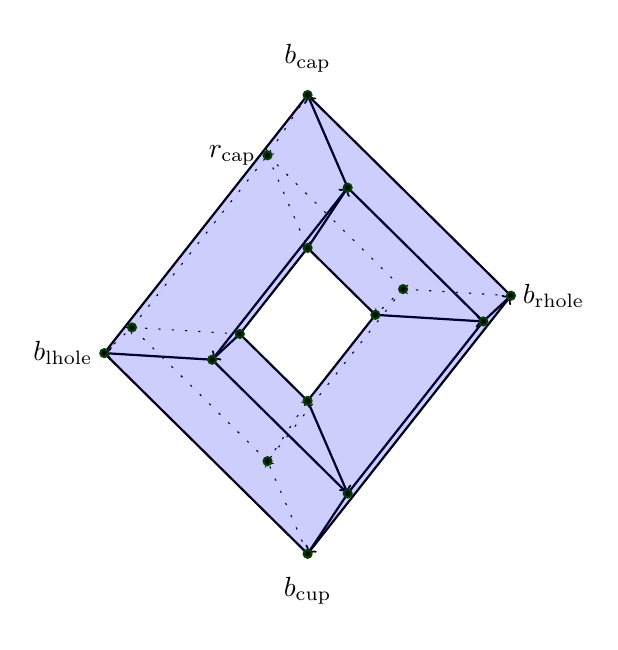
\begin{tikzpicture}%
  [x={(-0.860769cm, -0.121512cm)},
  y={(0.508996cm, -0.205391cm)},
  z={(-0.000053cm, 0.971107cm)},
  scale=1,
  back/.style={loosely dotted, thin},
  edge/.style={->,black, thick},
  line/.style={black, thick},
  facet/.style={fill=blue!95!black,fill opacity=0.1},
  vertex/.style={inner sep=1pt,circle,draw=green!25!black,fill=black,thick}]
\coordinate (r_cap) at (0, -1, 5);
\coordinate (g_cap) at (0, 0, 4 );
\coordinate (o_cap) at (0, 1, 5 );
\coordinate (b_cap) at (0, 0, 6 );

\coordinate (r_cup) at (0, -1, 1);
\coordinate (g_cup) at (0, 0, 2 );
\coordinate (o_cup) at (0, 1, 1 );
\coordinate (b_cup) at (0, 0, 0 );

\coordinate (r_ohole) at (-2, -1, 3);
\coordinate (g_ohole) at (-1, 0,  3);
\coordinate (o_ohole) at (-2, 1,  3);
\coordinate (b_ohole) at (-3, 0,  3);

\coordinate (r_rhole) at (2, -1, 3);
\coordinate (g_rhole) at (1, 0,  3);
\coordinate (o_rhole) at (2, 1,  3);
\coordinate (b_rhole) at (3, 0,  3);

\draw[edge,back] (r_cap) -- (g_cap);
\draw[edge]      (g_cap) -- (o_cap);
\draw[edge]      (o_cap) -- (b_cap);
\draw[edge,back] (b_cap) -- (r_cap);

\draw[edge,back] (r_cup) -- (g_cup);
\draw[edge]      (g_cup) -- (o_cup);
\draw[edge]      (o_cup) -- (b_cup);
\draw[edge,back] (b_cup) -- (r_cup);

\draw[edge,back] (r_ohole) -- (g_ohole);
\draw[edge]      (g_ohole) -- (o_ohole);
\draw[edge]      (o_ohole) -- (b_ohole);
\draw[edge,back] (b_ohole) -- (r_ohole);

\draw[edge,back] (r_rhole) -- (g_rhole);
\draw[edge]      (g_rhole) -- (o_rhole);
\draw[edge]      (o_rhole) -- (b_rhole);
\draw[edge,back] (b_rhole) -- (r_rhole);

\draw[line,back] (r_cap) --   (r_ohole);
\draw[line,back] (r_ohole) -- (r_cup);
\draw[line,back] (r_cup) --   (r_rhole);
\draw[line,back] (r_rhole) -- (r_cap);

\draw[line] (g_cap) --   (g_ohole);
\draw[line] (g_ohole) -- (g_cup);
\draw[line] (g_cup) --   (g_rhole);
\draw[line] (g_rhole) -- (g_cap);

\draw[line] (o_cap) --   (o_ohole);
\draw[line] (o_ohole) -- (o_cup);
\draw[line] (o_cup) --   (o_rhole);
\draw[line] (o_rhole) -- (o_cap);

\draw[line] (b_cap) --   (b_ohole);
\draw[line] (b_ohole) -- (b_cup);
\draw[line] (b_cup) --   (b_rhole);
\draw[line] (b_rhole) -- (b_cap);

\fill[facet] (r_cap) -- (r_ohole) -- (g_ohole) -- (g_cap) -- cycle {};
\fill[facet] (r_cap) -- (r_rhole) -- (g_rhole) -- (g_cap) -- cycle {};
\fill[facet] (r_cap) -- (r_ohole) -- (b_ohole) -- (b_cap) -- cycle {};
\fill[facet] (r_cap) -- (r_rhole) -- (b_rhole) -- (b_cap) -- cycle {};

\fill[facet] (o_cap) -- (o_ohole) -- (g_ohole) -- (g_cap) -- cycle {};
\fill[facet] (o_cap) -- (o_rhole) -- (g_rhole) -- (g_cap) -- cycle {};
\fill[facet] (o_cap) -- (o_ohole) -- (b_ohole) -- (b_cap) -- cycle {};
\fill[facet] (o_cap) -- (o_rhole) -- (b_rhole) -- (b_cap) -- cycle {};

\fill[facet] (r_cup) -- (r_ohole) -- (g_ohole) -- (g_cup) -- cycle {};
\fill[facet] (r_cup) -- (r_rhole) -- (g_rhole) -- (g_cup) -- cycle {};
\fill[facet] (r_cup) -- (r_ohole) -- (b_ohole) -- (b_cup) -- cycle {};
\fill[facet] (r_cup) -- (r_rhole) -- (b_rhole) -- (b_cup) -- cycle {};

\fill[facet] (o_cup) -- (o_ohole) -- (g_ohole) -- (g_cup) -- cycle {};
\fill[facet] (o_cup) -- (o_rhole) -- (g_rhole) -- (g_cup) -- cycle {};
\fill[facet] (o_cup) -- (o_ohole) -- (b_ohole) -- (b_cup) -- cycle {};
\fill[facet] (o_cup) -- (o_rhole) -- (b_rhole) -- (b_cup) -- cycle {};

\begin{scope}[nodes=vertex]
\node[label=left:\( r_{\mathrm{cap}} \)] at (r_cap) {};
\node at (g_cap) {};
\node at (o_cap) {};
\node[label=above:\( b_{\mathrm{cap}} \)] at (b_cap) {};
\node at (r_cup) {};
\node at (g_cup) {};
\node at (o_cup) {};
\node[label=below:\( b_{\mathrm{cup}} \)] at (b_cup) {};
\node at (r_ohole) {};
\node at (g_ohole) {};
\node at (o_ohole) {};
\node[label=right:\( b_{\mathrm{rhole}} \)] at (b_ohole) {};
\node at (r_rhole) {};
\node at (g_rhole) {};
\node at (o_rhole) {};
\node[label=left:\( b_{\mathrm{lhole}} \)] at (b_rhole) {};
\end{scope}
\end{tikzpicture}

\caption{Torus embedded in 3-dimensional space. If you see color in your rendering then black lines trace four square-shaped paths, red ones connect the front square to the middle diamonds, and blue ones connect the back path to the middle ones.}
\label{fig:torus}
\end{figure}

\begin{figure}[htbp]
\centering
% https://q.uiver.app/#q=WzAsMzYsWzEsNCwiXFxidWxsZXQiXSxbMSw2LCJcXGJ1bGxldCJdLFsyLDcsIlxcYnVsbGV0Il0sWzIsNSwiXFxidWxsZXQiXSxbMiwzLCJcXGJ1bGxldCJdLFsxLDgsIlxcYnVsbGV0Il0sWzEsMiwiXFxidWxsZXQiXSxbMywyLCJcXGJ1bGxldCJdLFszLDQsIlxcYnVsbGV0Il0sWzMsNiwiXFxidWxsZXQiXSxbMyw4LCJcXGJ1bGxldCJdLFsyLDEsIlxcYnVsbGV0Il0sWzQsMSwiXFxidWxsZXQiXSxbNSwyLCJcXGJ1bGxldCJdLFs0LDMsIlxcYnVsbGV0Il0sWzUsNCwiXFxidWxsZXQiXSxbNCw1LCJcXGJ1bGxldCJdLFs1LDYsIlxcYnVsbGV0Il0sWzQsNywiXFxidWxsZXQiXSxbNSw4LCJcXGJ1bGxldCJdLFsyLDAsIlxcbWF0aHJte2JhY2t9Il0sWzQsMCwiXFxtYXRocm17ZnJvbnR9Il0sWzEsMCwiXFxtYXRocm17b3V0ZXJ9Il0sWzMsMCwiXFxtYXRocm17aG9sZX0iXSxbNSwwLCJcXG1hdGhybXtvdXRlcn0iXSxbMSwxMCwiXFxidWxsZXQiXSxbMiw5LCJcXGJ1bGxldCJdLFszLDEwLCJcXGJ1bGxldCJdLFs0LDksIlxcYnVsbGV0Il0sWzUsMTAsIlxcYnVsbGV0Il0sWzAsMiwiXFxtYXRocm17dG9wXFwgb2ZcXCBkaWFtb25kc30iXSxbMCw2LCJcXG1hdGhybXtib3R0b21cXCBvZlxcIGRpYW1vbmRzfSJdLFsxLDEsIlxcICJdLFs1LDEsIlxcICJdLFszLDEsIlxcICJdLFswLDEwLCJcXG1hdGhybXt0b3BcXCBvZlxcIGRpYW1vbmRzfSJdLFs0LDMsIiIsMix7InN0eWxlIjp7ImhlYWQiOnsibmFtZSI6Im5vbmUifX19XSxbMywyLCIiLDIseyJzdHlsZSI6eyJoZWFkIjp7Im5hbWUiOiJub25lIn19fV0sWzAsMSwiIiwyLHsic3R5bGUiOnsiaGVhZCI6eyJuYW1lIjoibm9uZSJ9fX1dLFs0LDAsIiIsMSx7ImNvbG91ciI6WzIzNiw5MSw2MF0sInN0eWxlIjp7ImhlYWQiOnsibmFtZSI6Im5vbmUifX19XSxbMCwzLCIiLDEseyJjb2xvdXIiOlsyMzYsOTEsNjBdLCJzdHlsZSI6eyJoZWFkIjp7Im5hbWUiOiJub25lIn19fV0sWzMsMSwiIiwxLHsiY29sb3VyIjpbMjM2LDkxLDYwXSwic3R5bGUiOnsiaGVhZCI6eyJuYW1lIjoibm9uZSJ9fX1dLFsxLDIsIiIsMSx7ImNvbG91ciI6WzIzNiw5MSw2MF0sInN0eWxlIjp7ImhlYWQiOnsibmFtZSI6Im5vbmUifX19XSxbMiw1LCIiLDEseyJjb2xvdXIiOlsyMzYsOTEsNjBdLCJzdHlsZSI6eyJoZWFkIjp7Im5hbWUiOiJub25lIn19fV0sWzEsNSwiIiwxLHsic3R5bGUiOnsiaGVhZCI6eyJuYW1lIjoibm9uZSJ9fX1dLFs2LDQsIiIsMSx7ImNvbG91ciI6WzIzNiw5MSw2MF0sInN0eWxlIjp7ImhlYWQiOnsibmFtZSI6Im5vbmUifX19XSxbNiwwLCIiLDEseyJzdHlsZSI6eyJoZWFkIjp7Im5hbWUiOiJub25lIn19fV0sWzcsOCwiIiwwLHsic3R5bGUiOnsiaGVhZCI6eyJuYW1lIjoibm9uZSJ9fX1dLFs4LDksIiIsMCx7InN0eWxlIjp7ImhlYWQiOnsibmFtZSI6Im5vbmUifX19XSxbOSwxMCwiIiwwLHsic3R5bGUiOnsiaGVhZCI6eyJuYW1lIjoibm9uZSJ9fX1dLFs3LDQsIiIsMCx7ImNvbG91ciI6WzIzNiw5MSw2MF0sInN0eWxlIjp7ImhlYWQiOnsibmFtZSI6Im5vbmUifX19XSxbNCw4LCIiLDAseyJjb2xvdXIiOlsyMzYsOTEsNjBdLCJzdHlsZSI6eyJoZWFkIjp7Im5hbWUiOiJub25lIn19fV0sWzgsMywiIiwwLHsiY29sb3VyIjpbMjM2LDkxLDYwXSwic3R5bGUiOnsiaGVhZCI6eyJuYW1lIjoibm9uZSJ9fX1dLFszLDksIiIsMCx7ImNvbG91ciI6WzIzNiw5MSw2MF0sInN0eWxlIjp7ImhlYWQiOnsibmFtZSI6Im5vbmUifX19XSxbOSwyLCIiLDAseyJjb2xvdXIiOlsyMzYsOTEsNjBdLCJzdHlsZSI6eyJoZWFkIjp7Im5hbWUiOiJub25lIn19fV0sWzIsMTAsIiIsMCx7ImNvbG91ciI6WzIzNiw5MSw2MF0sInN0eWxlIjp7ImhlYWQiOnsibmFtZSI6Im5vbmUifX19XSxbMTEsNCwiIiwwLHsic3R5bGUiOnsiaGVhZCI6eyJuYW1lIjoibm9uZSJ9fX1dLFsxMSw2LCIiLDAseyJjb2xvdXIiOlsyMzYsOTEsNjBdLCJzdHlsZSI6eyJoZWFkIjp7Im5hbWUiOiJub25lIn19fV0sWzExLDcsIiIsMCx7ImNvbG91ciI6WzIzNiw5MSw2MF0sInN0eWxlIjp7ImhlYWQiOnsibmFtZSI6Im5vbmUifX19XSxbMTksMTcsIiIsMCx7InN0eWxlIjp7ImhlYWQiOnsibmFtZSI6Im5vbmUifX19XSxbMTgsMTYsIiIsMCx7InN0eWxlIjp7ImhlYWQiOnsibmFtZSI6Im5vbmUifX19XSxbMTYsMTQsIiIsMCx7InN0eWxlIjp7ImhlYWQiOnsibmFtZSI6Im5vbmUifX19XSxbMTcsMTUsIiIsMCx7InN0eWxlIjp7ImhlYWQiOnsibmFtZSI6Im5vbmUifX19XSxbMTUsMTMsIiIsMCx7InN0eWxlIjp7ImhlYWQiOnsibmFtZSI6Im5vbmUifX19XSxbMTQsMTIsIiIsMCx7InN0eWxlIjp7ImhlYWQiOnsibmFtZSI6Im5vbmUifX19XSxbMTIsNywiIiwwLHsiY29sb3VyIjpbMSw5NSw2MF0sInN0eWxlIjp7ImhlYWQiOnsibmFtZSI6Im5vbmUifX19XSxbMTIsMTMsIiIsMCx7ImNvbG91ciI6WzEsOTUsNjBdLCJzdHlsZSI6eyJoZWFkIjp7Im5hbWUiOiJub25lIn19fV0sWzEzLDE0LCIiLDAseyJjb2xvdXIiOlsxLDk1LDYwXSwic3R5bGUiOnsiaGVhZCI6eyJuYW1lIjoibm9uZSJ9fX1dLFsxNCw4LCIiLDAseyJjb2xvdXIiOlsxLDk1LDYwXSwic3R5bGUiOnsiaGVhZCI6eyJuYW1lIjoibm9uZSJ9fX1dLFsxNCwxNSwiIiwwLHsiY29sb3VyIjpbMSw5NSw2MF0sInN0eWxlIjp7ImhlYWQiOnsibmFtZSI6Im5vbmUifX19XSxbMTUsMTYsIiIsMCx7ImNvbG91ciI6WzEsOTUsNjBdLCJzdHlsZSI6eyJoZWFkIjp7Im5hbWUiOiJub25lIn19fV0sWzgsMTYsIiIsMCx7ImNvbG91ciI6WzEsOTUsNjBdLCJzdHlsZSI6eyJoZWFkIjp7Im5hbWUiOiJub25lIn19fV0sWzE2LDksIiIsMCx7ImNvbG91ciI6WzEsOTUsNjBdLCJzdHlsZSI6eyJoZWFkIjp7Im5hbWUiOiJub25lIn19fV0sWzE2LDE3LCIiLDAseyJjb2xvdXIiOlsxLDk1LDYwXSwic3R5bGUiOnsiaGVhZCI6eyJuYW1lIjoibm9uZSJ9fX1dLFsxNywxOCwiIiwwLHsiY29sb3VyIjpbMSw5NSw2MF0sInN0eWxlIjp7ImhlYWQiOnsibmFtZSI6Im5vbmUifX19XSxbOSwxOCwiIiwwLHsiY29sb3VyIjpbMSw5NSw2MF0sInN0eWxlIjp7ImhlYWQiOnsibmFtZSI6Im5vbmUifX19XSxbMTgsMTksIiIsMCx7ImNvbG91ciI6WzEsOTUsNjBdLCJzdHlsZSI6eyJoZWFkIjp7Im5hbWUiOiJub25lIn19fV0sWzE4LDEwLCIiLDAseyJjb2xvdXIiOlsxLDk1LDYwXSwic3R5bGUiOnsiaGVhZCI6eyJuYW1lIjoibm9uZSJ9fX1dLFs3LDE0LCIiLDAseyJjb2xvdXIiOlsxLDk1LDYwXSwic3R5bGUiOnsiaGVhZCI6eyJuYW1lIjoibm9uZSJ9fX1dLFs1LDI2LCIiLDEseyJjb2xvdXIiOlsyMzYsOTEsNjBdLCJzdHlsZSI6eyJoZWFkIjp7Im5hbWUiOiJub25lIn19fV0sWzEwLDI2LCIiLDEseyJjb2xvdXIiOlsyMzYsOTEsNjBdLCJzdHlsZSI6eyJoZWFkIjp7Im5hbWUiOiJub25lIn19fV0sWzIsMjYsIiIsMSx7InN0eWxlIjp7ImhlYWQiOnsibmFtZSI6Im5vbmUifX19XSxbMTgsMjgsIiIsMSx7InN0eWxlIjp7ImhlYWQiOnsibmFtZSI6Im5vbmUifX19XSxbMjYsMjUsIiIsMSx7ImNvbG91ciI6WzIzNiw5MSw2MF0sInN0eWxlIjp7ImhlYWQiOnsibmFtZSI6Im5vbmUifX19XSxbMjYsMjcsIiIsMSx7ImNvbG91ciI6WzIzNiw5MSw2MF0sInN0eWxlIjp7ImhlYWQiOnsibmFtZSI6Im5vbmUifX19XSxbMjgsMjksIiIsMSx7ImNvbG91ciI6WzEsOTUsNjBdLCJzdHlsZSI6eyJoZWFkIjp7Im5hbWUiOiJub25lIn19fV0sWzE5LDI5LCIiLDEseyJzdHlsZSI6eyJoZWFkIjp7Im5hbWUiOiJub25lIn19fV0sWzEwLDI3LCIiLDEseyJzdHlsZSI6eyJoZWFkIjp7Im5hbWUiOiJub25lIn19fV0sWzUsMjUsIiIsMSx7InN0eWxlIjp7ImhlYWQiOnsibmFtZSI6Im5vbmUifX19XSxbMjgsMjcsIiIsMSx7ImNvbG91ciI6WzEsOTUsNjBdLCJzdHlsZSI6eyJoZWFkIjp7Im5hbWUiOiJub25lIn19fV0sWzI4LDE5LCIiLDEseyJjb2xvdXIiOlsxLDk1LDYwXSwic3R5bGUiOnsiaGVhZCI6eyJuYW1lIjoibm9uZSJ9fX1dLFsyOCwxMCwiIiwxLHsiY29sb3VyIjpbMSw5NSw2MF0sInN0eWxlIjp7ImhlYWQiOnsibmFtZSI6Im5vbmUifX19XSxbMzAsNiwiIiwxLHsic3R5bGUiOnsiYm9keSI6eyJuYW1lIjoiZG90dGVkIn19fV0sWzMxLDEsIiIsMSx7InN0eWxlIjp7ImJvZHkiOnsibmFtZSI6ImRvdHRlZCJ9fX1dLFsyMCwxMSwiIiwwLHsic3R5bGUiOnsiYm9keSI6eyJuYW1lIjoiZG90dGVkIn19fV0sWzIxLDEyLCIiLDAseyJzdHlsZSI6eyJib2R5Ijp7Im5hbWUiOiJkb3R0ZWQifX19XSxbMjIsMzIsIiIsMCx7InN0eWxlIjp7ImJvZHkiOnsibmFtZSI6ImRvdHRlZCJ9fX1dLFsyNCwzMywiIiwwLHsic3R5bGUiOnsiYm9keSI6eyJuYW1lIjoiZG90dGVkIn19fV0sWzIzLDM0LCIiLDAseyJzdHlsZSI6eyJib2R5Ijp7Im5hbWUiOiJkb3R0ZWQifX19XSxbMzUsMjUsIiIsMSx7InN0eWxlIjp7ImJvZHkiOnsibmFtZSI6ImRvdHRlZCJ9fX1dXQ==
\begin{tikzcd}
	& {\mathrm{outer}} & {\mathrm{back}} & {\mathrm{hole}} & {\mathrm{front}} & {\mathrm{outer}} \\
	& {\ } & \bullet & {\ } & \bullet & {\ } \\
	{\mathrm{top\ of\ diamonds}} & \bullet && \bullet && \bullet \\
	&& \bullet && \bullet \\
	& \bullet && \bullet && \bullet \\
	&& \bullet && \bullet \\
	{\mathrm{bottom\ of\ diamonds}} & \bullet && \bullet && \bullet \\
	&& \bullet && \bullet \\
	& \bullet && \bullet && \bullet \\
	&& \bullet && \bullet \\
	{\mathrm{top\ of\ diamonds}} & \bullet && \bullet && \bullet
	\arrow[dotted, from=1-2, to=2-2]
	\arrow[dotted, from=1-3, to=2-3]
	\arrow[dotted, from=1-4, to=2-4]
	\arrow[dotted, from=1-5, to=2-5]
	\arrow[dotted, from=1-6, to=2-6]
	\arrow[draw={rgb,255:red,60;green,73;blue,246}, no head, from=2-3, to=3-2]
	\arrow[draw={rgb,255:red,60;green,73;blue,246}, no head, from=2-3, to=3-4]
	\arrow[no head, from=2-3, to=4-3]
	\arrow[draw={rgb,255:red,250;green,59;blue,56}, no head, from=2-5, to=3-4]
	\arrow[draw={rgb,255:red,250;green,59;blue,56}, no head, from=2-5, to=3-6]
	\arrow[dotted, from=3-1, to=3-2]
	\arrow[draw={rgb,255:red,60;green,73;blue,246}, no head, from=3-2, to=4-3]
	\arrow[no head, from=3-2, to=5-2]
	\arrow[draw={rgb,255:red,60;green,73;blue,246}, no head, from=3-4, to=4-3]
	\arrow[draw={rgb,255:red,250;green,59;blue,56}, no head, from=3-4, to=4-5]
	\arrow[no head, from=3-4, to=5-4]
	\arrow[draw={rgb,255:red,250;green,59;blue,56}, no head, from=3-6, to=4-5]
	\arrow[draw={rgb,255:red,60;green,73;blue,246}, no head, from=4-3, to=5-2]
	\arrow[draw={rgb,255:red,60;green,73;blue,246}, no head, from=4-3, to=5-4]
	\arrow[no head, from=4-3, to=6-3]
	\arrow[no head, from=4-5, to=2-5]
	\arrow[draw={rgb,255:red,250;green,59;blue,56}, no head, from=4-5, to=5-4]
	\arrow[draw={rgb,255:red,250;green,59;blue,56}, no head, from=4-5, to=5-6]
	\arrow[draw={rgb,255:red,60;green,73;blue,246}, no head, from=5-2, to=6-3]
	\arrow[no head, from=5-2, to=7-2]
	\arrow[draw={rgb,255:red,60;green,73;blue,246}, no head, from=5-4, to=6-3]
	\arrow[draw={rgb,255:red,250;green,59;blue,56}, no head, from=5-4, to=6-5]
	\arrow[no head, from=5-4, to=7-4]
	\arrow[no head, from=5-6, to=3-6]
	\arrow[draw={rgb,255:red,250;green,59;blue,56}, no head, from=5-6, to=6-5]
	\arrow[draw={rgb,255:red,60;green,73;blue,246}, no head, from=6-3, to=7-2]
	\arrow[draw={rgb,255:red,60;green,73;blue,246}, no head, from=6-3, to=7-4]
	\arrow[no head, from=6-3, to=8-3]
	\arrow[no head, from=6-5, to=4-5]
	\arrow[draw={rgb,255:red,250;green,59;blue,56}, no head, from=6-5, to=7-4]
	\arrow[draw={rgb,255:red,250;green,59;blue,56}, no head, from=6-5, to=7-6]
	\arrow[dotted, from=7-1, to=7-2]
	\arrow[draw={rgb,255:red,60;green,73;blue,246}, no head, from=7-2, to=8-3]
	\arrow[no head, from=7-2, to=9-2]
	\arrow[draw={rgb,255:red,60;green,73;blue,246}, no head, from=7-4, to=8-3]
	\arrow[draw={rgb,255:red,250;green,59;blue,56}, no head, from=7-4, to=8-5]
	\arrow[no head, from=7-4, to=9-4]
	\arrow[no head, from=7-6, to=5-6]
	\arrow[draw={rgb,255:red,250;green,59;blue,56}, no head, from=7-6, to=8-5]
	\arrow[draw={rgb,255:red,60;green,73;blue,246}, no head, from=8-3, to=9-2]
	\arrow[draw={rgb,255:red,60;green,73;blue,246}, no head, from=8-3, to=9-4]
	\arrow[no head, from=8-3, to=10-3]
	\arrow[no head, from=8-5, to=6-5]
	\arrow[draw={rgb,255:red,250;green,59;blue,56}, no head, from=8-5, to=9-4]
	\arrow[draw={rgb,255:red,250;green,59;blue,56}, no head, from=8-5, to=9-6]
	\arrow[no head, from=8-5, to=10-5]
	\arrow[color={rgb,255:red,60;green,73;blue,246}, no head, from=9-2, to=10-3]
	\arrow[no head, from=9-2, to=11-2]
	\arrow[color={rgb,255:red,60;green,73;blue,246}, no head, from=9-4, to=10-3]
	\arrow[no head, from=9-4, to=11-4]
	\arrow[no head, from=9-6, to=7-6]
	\arrow[no head, from=9-6, to=11-6]
	\arrow[color={rgb,255:red,60;green,73;blue,246}, no head, from=10-3, to=11-2]
	\arrow[color={rgb,255:red,60;green,73;blue,246}, no head, from=10-3, to=11-4]
	\arrow[color={rgb,255:red,250;green,59;blue,56}, no head, from=10-5, to=9-4]
	\arrow[color={rgb,255:red,250;green,59;blue,56}, no head, from=10-5, to=9-6]
	\arrow[color={rgb,255:red,250;green,59;blue,56}, no head, from=10-5, to=11-4]
	\arrow[color={rgb,255:red,250;green,59;blue,56}, no head, from=10-5, to=11-6]
	\arrow[dotted, from=11-1, to=11-2]
\end{tikzcd}

\caption{An inspiration for the torus. Identify the sides and then the top, definitionally, to get the actual torus.}
\label{fig:flattorus}
\end{figure}

This somewhat arbitrary and unfamiliar model of a torus has the helpful property that it is a combinatorial manifold that is somewhat minimal while still being representable by a donut shape. But the donut-shaped version suggests a very different connection than the flat model! Starting with the flat model, we can easily see how to define \( T_1 \) by sliding a link rigidly along the page to the link of some adjacent vertex. Then we can see that transport around any loop is the identity and so \( T_2 \) is always the identity (together with the homotopy \( \refl_\id \) from the identity to itself). So if we imagine a way to visit every face like we did for the octahedron, starting and ending at some basepoint \( v \), we expect to see no net rotation at all of \( Tv \). Later we will call this ``total curvature 0.''

The donut-shaped torus suggests a different connection, one determined by the embedding in 3-space that we have represented. But the easiest way to think about that bundle and its connection and curvature is to wait until we have a proof of the Poincaré-Hopf theorem, so that we can instead compute with a vector field.

\subsection{Vector fields}

\begin{mydef}
A \defemph{partial function} \( f:A\to B \) is a function \( f:A\to B+\star \), the disjoint union of \( B \) with the 1-element type.
\end{mydef}

If \( T:\mm\to\EMzo \) is a bundle of mere circles, then a vector field should be a partial function \( T_\bullet:\mm\to\EMpzo \) that lifts \( T \). In other words, a pointing of \emph{some} of the fibers. This aligns with the classical picture of a choice of nonzero vector at each point, except for some points where the vector field vanishes. So instead of having a notion corresponding to the full tangent vector space (one candidate for which would be the disk at each point, i.e. \( \link \) plus its spokes and filler triangles) we are mapping some vertices to their circular fibers, and others to \( \star \). This lets us continue to work with \( \EMzo \) instead of a type of tangent spaces.

Figure~\ref{fig:flattorus_zero} illustrates what removing the preimage of \( \star \) looks like. The resulting type is no longer a combinatorial manifold, since it fails the condition about every point having a circular link. 

\begin{figure}[htbp]
\centering
% https://q.uiver.app/#q=WzAsMzUsWzEsNCwiXFxidWxsZXQiXSxbMSw2LCJcXGJ1bGxldCJdLFsyLDcsIlxcYnVsbGV0Il0sWzIsNSwiXFxidWxsZXQiXSxbMiwzLCJcXGJ1bGxldCJdLFsxLDgsIlxcYnVsbGV0Il0sWzEsMiwiXFxidWxsZXQiXSxbMywyLCJcXGJ1bGxldCJdLFszLDQsIlxcYnVsbGV0Il0sWzMsOCwiXFxidWxsZXQiXSxbMiwxLCJcXGJ1bGxldCJdLFs0LDEsIlxcYnVsbGV0Il0sWzUsMiwiXFxidWxsZXQiXSxbNCwzLCJcXGJ1bGxldCJdLFs1LDQsIlxcYnVsbGV0Il0sWzQsNSwiXFxidWxsZXQiXSxbNSw2LCJcXGJ1bGxldCJdLFs0LDcsIlxcYnVsbGV0Il0sWzUsOCwiXFxidWxsZXQiXSxbMiwwLCJcXG1hdGhybXtiYWNrfSJdLFs0LDAsIlxcbWF0aHJte2Zyb250fSJdLFsxLDAsIlxcbWF0aHJte291dGVyfSJdLFszLDAsIlxcbWF0aHJte2hvbGV9Il0sWzUsMCwiXFxtYXRocm17b3V0ZXJ9Il0sWzEsMTAsIlxcYnVsbGV0Il0sWzIsOSwiXFxidWxsZXQiXSxbMywxMCwiXFxidWxsZXQiXSxbNCw5LCJcXGJ1bGxldCJdLFs1LDEwLCJcXGJ1bGxldCJdLFswLDIsIlxcbWF0aHJte3RvcFxcIG9mXFwgZGlhbW9uZHN9Il0sWzAsNiwiXFxtYXRocm17Ym90dG9tXFwgb2ZcXCBkaWFtb25kc30iXSxbMSwxLCJcXCAiXSxbNSwxLCJcXCAiXSxbMywxLCJcXCAiXSxbMCwxMCwiXFxtYXRocm17dG9wXFwgb2ZcXCBkaWFtb25kc30iXSxbNCwzLCIiLDIseyJzdHlsZSI6eyJoZWFkIjp7Im5hbWUiOiJub25lIn19fV0sWzMsMiwiIiwyLHsic3R5bGUiOnsiaGVhZCI6eyJuYW1lIjoibm9uZSJ9fX1dLFswLDEsIiIsMix7InN0eWxlIjp7ImhlYWQiOnsibmFtZSI6Im5vbmUifX19XSxbNCwwLCIiLDEseyJjb2xvdXIiOlsyMzYsOTEsNjBdLCJzdHlsZSI6eyJoZWFkIjp7Im5hbWUiOiJub25lIn19fV0sWzAsMywiIiwxLHsiY29sb3VyIjpbMjM2LDkxLDYwXSwic3R5bGUiOnsiaGVhZCI6eyJuYW1lIjoibm9uZSJ9fX1dLFszLDEsIiIsMSx7ImNvbG91ciI6WzIzNiw5MSw2MF0sInN0eWxlIjp7ImhlYWQiOnsibmFtZSI6Im5vbmUifX19XSxbMSwyLCIiLDEseyJjb2xvdXIiOlsyMzYsOTEsNjBdLCJzdHlsZSI6eyJoZWFkIjp7Im5hbWUiOiJub25lIn19fV0sWzIsNSwiIiwxLHsiY29sb3VyIjpbMjM2LDkxLDYwXSwic3R5bGUiOnsiaGVhZCI6eyJuYW1lIjoibm9uZSJ9fX1dLFsxLDUsIiIsMSx7InN0eWxlIjp7ImhlYWQiOnsibmFtZSI6Im5vbmUifX19XSxbNiw0LCIiLDEseyJjb2xvdXIiOlsyMzYsOTEsNjBdLCJzdHlsZSI6eyJoZWFkIjp7Im5hbWUiOiJub25lIn19fV0sWzYsMCwiIiwxLHsic3R5bGUiOnsiaGVhZCI6eyJuYW1lIjoibm9uZSJ9fX1dLFs3LDgsIiIsMCx7InN0eWxlIjp7ImhlYWQiOnsibmFtZSI6Im5vbmUifX19XSxbNyw0LCIiLDAseyJjb2xvdXIiOlsyMzYsOTEsNjBdLCJzdHlsZSI6eyJoZWFkIjp7Im5hbWUiOiJub25lIn19fV0sWzQsOCwiIiwwLHsiY29sb3VyIjpbMjM2LDkxLDYwXSwic3R5bGUiOnsiaGVhZCI6eyJuYW1lIjoibm9uZSJ9fX1dLFs4LDMsIiIsMCx7ImNvbG91ciI6WzIzNiw5MSw2MF0sInN0eWxlIjp7ImhlYWQiOnsibmFtZSI6Im5vbmUifX19XSxbMiw5LCIiLDAseyJjb2xvdXIiOlsyMzYsOTEsNjBdLCJzdHlsZSI6eyJoZWFkIjp7Im5hbWUiOiJub25lIn19fV0sWzEwLDQsIiIsMCx7InN0eWxlIjp7ImhlYWQiOnsibmFtZSI6Im5vbmUifX19XSxbMTAsNiwiIiwwLHsiY29sb3VyIjpbMjM2LDkxLDYwXSwic3R5bGUiOnsiaGVhZCI6eyJuYW1lIjoibm9uZSJ9fX1dLFsxMCw3LCIiLDAseyJjb2xvdXIiOlsyMzYsOTEsNjBdLCJzdHlsZSI6eyJoZWFkIjp7Im5hbWUiOiJub25lIn19fV0sWzE4LDE2LCIiLDAseyJzdHlsZSI6eyJoZWFkIjp7Im5hbWUiOiJub25lIn19fV0sWzE3LDE1LCIiLDAseyJzdHlsZSI6eyJoZWFkIjp7Im5hbWUiOiJub25lIn19fV0sWzE1LDEzLCIiLDAseyJzdHlsZSI6eyJoZWFkIjp7Im5hbWUiOiJub25lIn19fV0sWzE2LDE0LCIiLDAseyJzdHlsZSI6eyJoZWFkIjp7Im5hbWUiOiJub25lIn19fV0sWzE0LDEyLCIiLDAseyJzdHlsZSI6eyJoZWFkIjp7Im5hbWUiOiJub25lIn19fV0sWzEzLDExLCIiLDAseyJzdHlsZSI6eyJoZWFkIjp7Im5hbWUiOiJub25lIn19fV0sWzExLDcsIiIsMCx7ImNvbG91ciI6WzEsOTUsNjBdLCJzdHlsZSI6eyJoZWFkIjp7Im5hbWUiOiJub25lIn19fV0sWzExLDEyLCIiLDAseyJjb2xvdXIiOlsxLDk1LDYwXSwic3R5bGUiOnsiaGVhZCI6eyJuYW1lIjoibm9uZSJ9fX1dLFsxMiwxMywiIiwwLHsiY29sb3VyIjpbMSw5NSw2MF0sInN0eWxlIjp7ImhlYWQiOnsibmFtZSI6Im5vbmUifX19XSxbMTMsOCwiIiwwLHsiY29sb3VyIjpbMSw5NSw2MF0sInN0eWxlIjp7ImhlYWQiOnsibmFtZSI6Im5vbmUifX19XSxbMTMsMTQsIiIsMCx7ImNvbG91ciI6WzEsOTUsNjBdLCJzdHlsZSI6eyJoZWFkIjp7Im5hbWUiOiJub25lIn19fV0sWzE0LDE1LCIiLDAseyJjb2xvdXIiOlsxLDk1LDYwXSwic3R5bGUiOnsiaGVhZCI6eyJuYW1lIjoibm9uZSJ9fX1dLFs4LDE1LCIiLDAseyJjb2xvdXIiOlsxLDk1LDYwXSwic3R5bGUiOnsiaGVhZCI6eyJuYW1lIjoibm9uZSJ9fX1dLFsxNSwxNiwiIiwwLHsiY29sb3VyIjpbMSw5NSw2MF0sInN0eWxlIjp7ImhlYWQiOnsibmFtZSI6Im5vbmUifX19XSxbMTYsMTcsIiIsMCx7ImNvbG91ciI6WzEsOTUsNjBdLCJzdHlsZSI6eyJoZWFkIjp7Im5hbWUiOiJub25lIn19fV0sWzE3LDE4LCIiLDAseyJjb2xvdXIiOlsxLDk1LDYwXSwic3R5bGUiOnsiaGVhZCI6eyJuYW1lIjoibm9uZSJ9fX1dLFsxNyw5LCIiLDAseyJjb2xvdXIiOlsxLDk1LDYwXSwic3R5bGUiOnsiaGVhZCI6eyJuYW1lIjoibm9uZSJ9fX1dLFs3LDEzLCIiLDAseyJjb2xvdXIiOlsxLDk1LDYwXSwic3R5bGUiOnsiaGVhZCI6eyJuYW1lIjoibm9uZSJ9fX1dLFs1LDI1LCIiLDEseyJjb2xvdXIiOlsyMzYsOTEsNjBdLCJzdHlsZSI6eyJoZWFkIjp7Im5hbWUiOiJub25lIn19fV0sWzksMjUsIiIsMSx7ImNvbG91ciI6WzIzNiw5MSw2MF0sInN0eWxlIjp7ImhlYWQiOnsibmFtZSI6Im5vbmUifX19XSxbMiwyNSwiIiwxLHsic3R5bGUiOnsiaGVhZCI6eyJuYW1lIjoibm9uZSJ9fX1dLFsxNywyNywiIiwxLHsic3R5bGUiOnsiaGVhZCI6eyJuYW1lIjoibm9uZSJ9fX1dLFsyNSwyNCwiIiwxLHsiY29sb3VyIjpbMjM2LDkxLDYwXSwic3R5bGUiOnsiaGVhZCI6eyJuYW1lIjoibm9uZSJ9fX1dLFsyNSwyNiwiIiwxLHsiY29sb3VyIjpbMjM2LDkxLDYwXSwic3R5bGUiOnsiaGVhZCI6eyJuYW1lIjoibm9uZSJ9fX1dLFsyNywyOCwiIiwxLHsiY29sb3VyIjpbMSw5NSw2MF0sInN0eWxlIjp7ImhlYWQiOnsibmFtZSI6Im5vbmUifX19XSxbMTgsMjgsIiIsMSx7InN0eWxlIjp7ImhlYWQiOnsibmFtZSI6Im5vbmUifX19XSxbOSwyNiwiIiwxLHsic3R5bGUiOnsiaGVhZCI6eyJuYW1lIjoibm9uZSJ9fX1dLFs1LDI0LCIiLDEseyJzdHlsZSI6eyJoZWFkIjp7Im5hbWUiOiJub25lIn19fV0sWzI3LDI2LCIiLDEseyJjb2xvdXIiOlsxLDk1LDYwXSwic3R5bGUiOnsiaGVhZCI6eyJuYW1lIjoibm9uZSJ9fX1dLFsyNywxOCwiIiwxLHsiY29sb3VyIjpbMSw5NSw2MF0sInN0eWxlIjp7ImhlYWQiOnsibmFtZSI6Im5vbmUifX19XSxbMjcsOSwiIiwxLHsiY29sb3VyIjpbMSw5NSw2MF0sInN0eWxlIjp7ImhlYWQiOnsibmFtZSI6Im5vbmUifX19XSxbMjksNiwiIiwxLHsic3R5bGUiOnsiYm9keSI6eyJuYW1lIjoiZG90dGVkIn19fV0sWzMwLDEsIiIsMSx7InN0eWxlIjp7ImJvZHkiOnsibmFtZSI6ImRvdHRlZCJ9fX1dLFsxOSwxMCwiIiwwLHsic3R5bGUiOnsiYm9keSI6eyJuYW1lIjoiZG90dGVkIn19fV0sWzIwLDExLCIiLDAseyJzdHlsZSI6eyJib2R5Ijp7Im5hbWUiOiJkb3R0ZWQifX19XSxbMjEsMzEsIiIsMCx7InN0eWxlIjp7ImJvZHkiOnsibmFtZSI6ImRvdHRlZCJ9fX1dLFsyMywzMiwiIiwwLHsic3R5bGUiOnsiYm9keSI6eyJuYW1lIjoiZG90dGVkIn19fV0sWzIyLDMzLCIiLDAseyJzdHlsZSI6eyJib2R5Ijp7Im5hbWUiOiJkb3R0ZWQifX19XSxbMzQsMjQsIiIsMSx7InN0eWxlIjp7ImJvZHkiOnsibmFtZSI6ImRvdHRlZCJ9fX1dXQ==
\begin{tikzcd}[column sep=1ex,row sep=1ex]
  & {\mathrm{outer}} & {\mathrm{back}} & {\mathrm{hole}} & {\mathrm{front}} & {\mathrm{outer}} \\
  & {\ } & \bullet & {\ } & \bullet & {\ } \\
  {\mathrm{top\ of\ diamonds}} & \bullet && \bullet && \bullet \\
  && \bullet && \bullet \\
  & \bullet && \bullet && \bullet \\
  && \bullet && \bullet \\
  {\mathrm{bottom\ of\ diamonds}} & \bullet &&&& \bullet \\
  && \bullet && \bullet \\
  & \bullet && \bullet && \bullet \\
  && \bullet && \bullet \\
  {\mathrm{top\ of\ diamonds}} & \bullet && \bullet && \bullet
  \arrow[dotted, from=1-2, to=2-2]
  \arrow[dotted, from=1-3, to=2-3]
  \arrow[dotted, from=1-4, to=2-4]
  \arrow[dotted, from=1-5, to=2-5]
  \arrow[dotted, from=1-6, to=2-6]
  \arrow[draw={rgb,255:red,60;green,73;blue,246}, no head, from=2-3, to=3-2]
  \arrow[draw={rgb,255:red,60;green,73;blue,246}, no head, from=2-3, to=3-4]
  \arrow[no head, from=2-3, to=4-3]
  \arrow[draw={rgb,255:red,250;green,59;blue,56}, no head, from=2-5, to=3-4]
  \arrow[draw={rgb,255:red,250;green,59;blue,56}, no head, from=2-5, to=3-6]
  \arrow[dotted, from=3-1, to=3-2]
  \arrow[draw={rgb,255:red,60;green,73;blue,246}, no head, from=3-2, to=4-3]
  \arrow[no head, from=3-2, to=5-2]
  \arrow[draw={rgb,255:red,60;green,73;blue,246}, no head, from=3-4, to=4-3]
  \arrow[draw={rgb,255:red,250;green,59;blue,56}, no head, from=3-4, to=4-5]
  \arrow[no head, from=3-4, to=5-4]
  \arrow[draw={rgb,255:red,250;green,59;blue,56}, no head, from=3-6, to=4-5]
  \arrow[draw={rgb,255:red,60;green,73;blue,246}, no head, from=4-3, to=5-2]
  \arrow[draw={rgb,255:red,60;green,73;blue,246}, no head, from=4-3, to=5-4]
  \arrow[no head, from=4-3, to=6-3]
  \arrow[no head, from=4-5, to=2-5]
  \arrow[draw={rgb,255:red,250;green,59;blue,56}, no head, from=4-5, to=5-4]
  \arrow[draw={rgb,255:red,250;green,59;blue,56}, no head, from=4-5, to=5-6]
  \arrow[draw={rgb,255:red,60;green,73;blue,246}, no head, from=5-2, to=6-3]
  \arrow[no head, from=5-2, to=7-2]
  \arrow[draw={rgb,255:red,60;green,73;blue,246}, no head, from=5-4, to=6-3]
  \arrow[draw={rgb,255:red,250;green,59;blue,56}, no head, from=5-4, to=6-5]
  \arrow[no head, from=5-6, to=3-6]
  \arrow[draw={rgb,255:red,250;green,59;blue,56}, no head, from=5-6, to=6-5]
  \arrow[draw={rgb,255:red,60;green,73;blue,246}, no head, from=6-3, to=7-2]
  \arrow[no head, from=6-3, to=8-3]
  \arrow[no head, from=6-5, to=4-5]
  \arrow[draw={rgb,255:red,250;green,59;blue,56}, no head, from=6-5, to=7-6]
  \arrow[dotted, from=7-1, to=7-2]
  \arrow[draw={rgb,255:red,60;green,73;blue,246}, no head, from=7-2, to=8-3]
  \arrow[no head, from=7-2, to=9-2]
  \arrow[no head, from=7-6, to=5-6]
  \arrow[draw={rgb,255:red,250;green,59;blue,56}, no head, from=7-6, to=8-5]
  \arrow[draw={rgb,255:red,60;green,73;blue,246}, no head, from=8-3, to=9-2]
  \arrow[draw={rgb,255:red,60;green,73;blue,246}, no head, from=8-3, to=9-4]
  \arrow[no head, from=8-3, to=10-3]
  \arrow[no head, from=8-5, to=6-5]
  \arrow[draw={rgb,255:red,250;green,59;blue,56}, no head, from=8-5, to=9-4]
  \arrow[draw={rgb,255:red,250;green,59;blue,56}, no head, from=8-5, to=9-6]
  \arrow[no head, from=8-5, to=10-5]
  \arrow[draw={rgb,255:red,60;green,73;blue,246}, no head, from=9-2, to=10-3]
  \arrow[no head, from=9-2, to=11-2]
  \arrow[draw={rgb,255:red,60;green,73;blue,246}, no head, from=9-4, to=10-3]
  \arrow[no head, from=9-4, to=11-4]
  \arrow[no head, from=9-6, to=7-6]
  \arrow[no head, from=9-6, to=11-6]
  \arrow[draw={rgb,255:red,60;green,73;blue,246}, no head, from=10-3, to=11-2]
  \arrow[draw={rgb,255:red,60;green,73;blue,246}, no head, from=10-3, to=11-4]
  \arrow[draw={rgb,255:red,250;green,59;blue,56}, no head, from=10-5, to=9-4]
  \arrow[draw={rgb,255:red,250;green,59;blue,56}, no head, from=10-5, to=9-6]
  \arrow[draw={rgb,255:red,250;green,59;blue,56}, no head, from=10-5, to=11-4]
  \arrow[draw={rgb,255:red,250;green,59;blue,56}, no head, from=10-5, to=11-6]
  \arrow[dotted, from=11-1, to=11-2]
\end{tikzcd}
\caption{The flat torus with one vertex removed. This also removes the edges and faces containing that vertex.}
\label{fig:flattorus_zero}
\end{figure}

\begin{mydef}
Let \( \mm:\combmfdt \) be a combinatorial manifold and \( Z \) an isolated set of vertices. A \defemph{vector field \( X \) on \( \mm \) with zero set \( Z \)} is a partial section of \( P \), i.e. a term \( X:\pit{x:\mm\setminus Z}T(x) \) (and eliding the unique term of \( Z\to\star \)). The \defemph{exponential map} \( \exp:P\to \mm \) is the map sending points in a fiber to the corresponding point in the link of the base point: \( \exp(x, y:\link(x))=y \). In commutative diagram form we have:
\end{mydef}
% https://q.uiver.app/#q=WzAsNCxbMCwyLCJNXFxzZXRtaW51cyBaIl0sWzIsMiwiXFxtYXRocm17RU19KFxcbWF0aGJie1p9LDEpIl0sWzIsMCwiXFxtYXRocm17RU19X1xcYnVsbGV0KFxcbWF0aGJie1p9LDEpIl0sWzAsMCwiUFxcc3RhY2tyZWx7XFxtYXRocm17ZGVmfX09e1xcc3VtX3tDOlRNfUN9Il0sWzAsMSwiVCJdLFsyLDEsIlxcbWF0aHJte3ByfV8xIl0sWzMsMCwiXFxtYXRocm17cHJ9XzEiXSxbMywyLCJcXG92ZXJsaW5le1R9Il0sWzAsMywie1g6XFxwcm9kX3t4Ok1cXHNldG1pbnVzIFp9VHh9IiwwLHsiY3VydmUiOi0zfV0sWzMsMCwiXFxtYXRocm17ZXhwfSIsMCx7ImN1cnZlIjotM31dLFswLDIsIlRfXFxidWxsZXQiXSxbMywxLCIiLDAseyJzdHlsZSI6eyJuYW1lIjoiY29ybmVyIn19XV0=
\begin{center}
\begin{tikzcd}
  {P\stackrel{\mathrm{def}}={\sum_{C:T(\mm\setminus Z)}C}} && {\mathrm{EM}_\bullet(\mathbb{Z},1)} \\
  \\
  {\mm\setminus Z} && {\mathrm{EM}(\mathbb{Z},1)}
  \arrow["{\overline{T}}", from=1-1, to=1-3]
  \arrow["{\mathrm{pr}_1}", from=1-1, to=3-1]
  \arrow["{\mathrm{exp}}", curve={height=-18pt}, from=1-1, to=3-1]
  \arrow["\lrcorner"{anchor=center, pos=0.125}, draw=none, from=1-1, to=3-3]
  \arrow["{\mathrm{pr}_1}", from=1-3, to=3-3]
  \arrow["{{X:\prod_{x:\mm\setminus Z}Tx}}", curve={height=-18pt}, from=3-1, to=1-1]
  \arrow["{T_\bullet}", from=3-1, to=1-3]
  \arrow["T", from=3-1, to=3-3]
\end{tikzcd}
\end{center}
where \( T_\bullet=\overline{T}\circ X \). Note that \( \exp \) is different from \( \pr_1 \) since it spreads a fiber out onto the manifold. The composition \( \exp\circ X \) is a map \( \mm\setminus Z\to \mm \), and can be thought of as the flow of the vector field.

Let's see a few examples.

\begin{mydef}
The \defemph{spinning vector field} \( \Xspin \) on \( \oo\setminus\{w, y\} \) is given by the following data. We compose with \( \exp \) to keep the notation directly in \( \oo \). See Figure~\ref{fig:sphere_spin}
\begin{align*}
\exp\circ\Xspin(b)  &=r   \\
\exp\circ\Xspin(r)  &=g   \\
\exp\circ\Xspin(g)  &=o   \\
\exp\circ\Xspin(o)  &=b   \\
\end{align*}
We must also define pathovers and faceovers, i.e. \( \apd(\Xspin \). For example, \( \Xspin(b) \) is the point \( r \) in the link \( woyr \). Transport along \( br \) takes the link of \( b \) to the link of \( r \), mapping \( r:Tb \) to \( g:Tr \). This agrees with \( \Xspin(r) \) and so we will choose \( \Xspin(br)=\refl_g \) in \( Tr \). We similarly choose \( \refl \) pathovers for the other equatorial edges. And since we have deleted all the faces when removing the zeros, there are no faceovers.
\end{mydef}

\begin{figure}[htbp]
\centering
\begin{tikzpicture}%
  [x={(-0.860769cm, -0.121512cm)},
  y={(0.508996cm, -0.205391cm)},
  z={(-0.000053cm, 0.971107cm)},
  scale=1,
  eqback/.style={-Latex, very thick},
  back/.style={loosely dotted, thin},
  eqedge/.style={-Latex, very thick},
  edge/.style={black, thin},
  facet/.style={fill=blue!95!black,fill opacity=0.0},
  vertex/.style={inner sep=1pt,circle,draw=green!25!black,fill=black,thick}]
\coordinate (-1, -1, 0) at (-1, -1, 0);
\coordinate (-1, 1, 0) at (-1, 1, 0);
\coordinate (0, 0, -1) at (0, 0, -1);
\coordinate (0, 0, 1) at (0, 0, 1);
\coordinate (1, -1, 0) at (1, -1, 0);
\coordinate (1, 1, 0) at (1, 1, 0);
%% Drawing edges in the back
%%
\draw[edge,eqback] (-1, -1, 0) -- (-1, 1, 0);
\draw[edge,back] (-1, -1, 0) -- (0, 0, -1.4);
\draw[edge,back] (-1, -1, 0) -- (0, 0, 1.4);
\draw[edge,eqback] (1, -1, 0) -- (-1, -1, 0);
%% Drawing vertices in the back
%%
\node[vertex] at (-1, -1, 0)     {};
%% Drawing the facets
%%
\fill[facet] (1, 1, 0) -- (0, 0, -1.4) -- (1, -1, 0) -- cycle {};
\fill[facet] (1, 1, 0) -- (0, 0, 1.4) -- (1, -1, 0) -- cycle {};
\fill[facet] (1, 1, 0) -- (-1, 1, 0) -- (0, 0, 1.4) -- cycle {};
\fill[facet] (1, 1, 0) -- (-1, 1, 0) -- (0, 0, -1.4) -- cycle {};
%% Drawing edges in the front
%%
\draw[edge] (-1, 1, 0) -- (0, 0, -1.4);
\draw[edge] (-1, 1, 0) -- (0, 0, 1.4);
\draw[eqedge] (-1, 1, 0) -- (1, 1, 0);
\draw[edge] (0, 0, -1.4) -- (1, -1, 0);
\draw[edge] (0, 0, -1.4) -- (1, 1, 0);
\draw[edge] (0, 0, 1.4) -- (1, -1, 0);
\draw[edge] (0, 0, 1.4) -- (1, 1, 0);
\draw[eqedge] (1, 1, 0) -- (1, -1, 0);
%% Drawing the vertices in the front
%%
\begin{scope}[nodes=vertex]
\node[label=above right:\( b \)] at (-1, 1, 0)     {};
\node[label=below:\( y \)] at (0, 0, -1.4)     {};
\node[label=above:\( w \)] at (0, 0, 1.4)     {};
\node[label=above left:\( g \)] at (1, -1, 0)     {};
\node[label=above left:\( r \)] at (1, 1, 0)     {};
\node[label=above right:\( o \)] at (-1, -1, 0)     {};
\end{scope}
\end{tikzpicture}
\caption{The vector field \( \Xspin \) on \( \oo \), which circulates around the equator. \( w \) and \( y \) are zeros.}
\label{fig:sphere_spin}
\end{figure}%fig:sphere_spin

\begin{mydef}
The \defemph{downward vector field} \( \Xdown \) on \( \oo\setminus\{w, y\} \) is given by the following data, where again we compose with \( \exp \) to keep the notation directly in \( \oo \). See Figure~\ref{fig:sphere_downward}
\begin{align*}
\exp\circ\Xspin(b)  &=y   \\
\exp\circ\Xspin(r)  &=y   \\
\exp\circ\Xspin(g)  &=y   \\
\exp\circ\Xspin(o)  &=y   \\
\end{align*}
We also need to select a pathover for each edge on the equator. Transport on all these edges takes \( y \) in one fiber to \( y \) in the next, so we choose the path \( \refl_y\) in all four of these fibers. Again there are no faceovers to map.
\end{mydef}

\begin{figure}[htbp]
\centering
\begin{tikzpicture}%
  [x={(-0.860769cm, -0.121512cm)},
  y={(0.508996cm, -0.205391cm)},
  z={(-0.000053cm, 0.971107cm)},
  scale=1,
  eqback/.style={-Latex, very thick},
  back/.style={loosely dotted, thin},
  eqedge/.style={-Latex, very thick},
  edge/.style={black, thin},
  facet/.style={fill=blue!95!black,fill opacity=0.0},
  vertex/.style={inner sep=1pt,circle,draw=green!25!black,fill=black,thick}]
\coordinate (-1, -1, 0) at (-1, -1, 0);
\coordinate (-1, 1, 0) at (-1, 1, 0);
\coordinate (0, 0, -1) at (0, 0, -1);
\coordinate (0, 0, 1) at (0, 0, 1);
\coordinate (1, -1, 0) at (1, -1, 0);
\coordinate (1, 1, 0) at (1, 1, 0);
%% Drawing edges in the back
%%
\draw[edge,back] (-1, -1, 0) -- (-1, 1, 0);
\draw[eqedge] (-1, -1, 0) -- (0, 0, -1.4);
\draw[edge,back] (-1, -1, 0) -- (0, 0, 1.4);
\draw[edge,back] (1, -1, 0) -- (-1, -1, 0);
%% Drawing vertices in the back
%%
\node[vertex] at (-1, -1, 0)     {};
%% Drawing the facets
%%
\fill[facet] (1, 1, 0) -- (0, 0, -1.4) -- (1, -1, 0) -- cycle {};
\fill[facet] (1, 1, 0) -- (0, 0, 1.4) -- (1, -1, 0) -- cycle {};
\fill[facet] (1, 1, 0) -- (-1, 1, 0) -- (0, 0, 1.4) -- cycle {};
\fill[facet] (1, 1, 0) -- (-1, 1, 0) -- (0, 0, -1.4) -- cycle {};
%% Drawing edges in the front
%%
\draw[eqedge] (-1, 1, 0) -- (0, 0, -1.4);
\draw[edge] (-1, 1, 0) -- (0, 0, 1.4);
\draw[edge] (-1, 1, 0) -- (1, 1, 0);
\draw[eqedge] (1, -1, 0) -- (0, 0, -1.4);
\draw[eqedge] (1, 1, 0) -- (0, 0, -1.4);
\draw[edge] (0, 0, 1.4) -- (1, -1, 0);
\draw[edge] (0, 0, 1.4) -- (1, 1, 0);
\draw[edge] (1, 1, 0) -- (1, -1, 0);
%% Drawing the vertices in the front
%%
\begin{scope}[nodes=vertex]
\node[label=above right:\( b \)] at (-1, 1, 0)     {};
\node[label=below:\( y \)] at (0, 0, -1.4)     {};
\node[label=above:\( w \)] at (0, 0, 1.4)     {};
\node[label=above left:\( g \)] at (1, -1, 0)     {};
\node[label=above left:\( r \)] at (1, 1, 0)     {};
\node[label=above right:\( o \)] at (-1, -1, 0)     {};
\end{scope}
\end{tikzpicture}
\caption{The vector field \( \Xdown \) on \( \oo \), which flows downward. \( w \) and \( y \) are zeros.}
\label{fig:sphere_downward}
\end{figure}%fig:sphere_downward

\subsection{Index of a vector field}

Index should be an integer that computes a winding number ``of the vector field'' around a zero. We can compute an integer from a map by taking its \emph{degree}, which is a construction we will assume that we have, for example using \cite{buchholtz_favonia}, where they indeed require that degree agrees with winding number for maps \( S^1\to S^1 \).

\begin{mydef}
Let \( \mm:\combmfdt \) and let \( T:\mm\to\EMzo \) be a bundle of circles given on \( \mm_0 \) by \( \link \). Let \( z:Z \) be an isolated zero and let \( \link z \) be its polygonal link in \( \mm \), with a clockwise orientation, say with ordered vertices \( \{l_{z1},\ldots,l_{zn}\} \). We call the degree of the map \( \tr(\link z):Tl_{z1}=Tl_{z1} \) the \defemph{index of \( X \) at \( z \)}. It does not depend on which vertex we use.
\end{mydef}

% \begin{mydef}
% Let \( \mm:\combmfdt \), let \( T:\mm\to\EMzo \) be the discrete tangent bundle given on \( \mm_0 \) by \( \link \). Let \( P\defeq\sit{x:\mm}Tx \), and \( Z \) be a set of isolated zeros. Let \( X:\mm\setminus Z\to P \) be a nonvanishing vector field. Finally, let \( z:Z \) be a zero and let \( \link z \) be its polygonal link in \( \mm \), with a clockwise orientation, say with ordered vertices \( \{l_{z1},\ldots,l_{zn}\} \). Define a map \( X'(z):\link z\to \link z \), called \defemph{the circle automorphism at \( z \)}, on vertices of \( \link z \) as follows:
% \[ 
% X'(z)(l_{zi}) = \exp\left(\tr(l_{zi}z)(X(l_{zi})\right) 
% \] In words, we transport the vector field along the unique edge joining \( l_{zi} \) to \( z \), then apply \( \exp \). The result will be some point in \( \link z \). In different words, \( X(l_{zi}) \) may point various places: to another point of \( \link z \), to \( z \) itself, or somewhere beyond \( \link z \). Transporting all these fibers to the central fiber at \( z \), then exponentiating, gives a self-map of the link.
% 
% \( X'(z) \) extends to the edges of \( \link z \), e.g. \( l_{z1}l_{z2} \), by the action on paths of \( \tr \) along \( l_{zi}z \). To visualize this we can imagine transporting \( X \) along an edge of \( \link z \) from \( l_{z1} \) to \( l_{z2} \) and then transporting the result along \( l_{z2}z \).
% 
% Finally, we call the degree of \( X'(z) \) on the clockwise-oriented link the \defemph{index of \( X \) at \( z \)}.\qed
% \end{mydef}

\begin{mylemma}
The index of \( \Xspin \) at both \( y \) and at \( w \) is 1, and the same is true for \( \Xdown \).
\end{mylemma}
\begin{proof}
\( \apd(\Xspin)(br) = \refl_{\Xspin(r)} \) and similarly for the other edges and for \( \Xdown \). So \( \apd \) on the loop around the equator is the identity, which has index 1.
\end{proof}

If these vector fields both have index +1, what does index --1 look like? We can see an example on the torus with its downward vector field.

On the torus we can also consider both a spinning vector field and a downward vector field. Figure~\ref{fig:spin_torus} shows one way to spin the torus, and in this case there are no zeros so the index is the degree of a map from the empty set, which is 0 (as it factors through a constant map).

Figure~\ref{fig:morse_torus} shows a downward flow with four zeros. Although this is a picture of the flat torus, the vector field is derived from the shape of Figure~\ref{fig:torus} where we actually have a notion of up and down. We see at the position labeled (outer, top of diamonds), i.e. the top of the torus, an everywhere outward pointing vector field. At (outer, bottom of diamonds) we see an inward pointing vector field. But at (hole, top of diamonds), i.e. the top of the hole, we see something else. Imagine transport from the neighbor to the lower right to the neighbor below, then continuing clockwise around the link. If we assume that we define \( \apd \) on these edges to be \emph{counterclockwise} rotation, then transport around the whole link has degree --1. Similarly for the zero at (hole, bottom of diamonds). Adding these four indexes we again get 0.

Summarizing what we've seen in our examples, vector fields with isolated zeros have an index, and this index tracks with the total curvature, and the Euler characteristic.

\begin{figure}[htbp]
\centering
\begin{tikzcd}[column sep=1ex,row sep=1ex]
  & {\mathrm{outer}} & {\mathrm{back}} & {\mathrm{hole}} & {\mathrm{front}} & {\mathrm{outer}} \\
  & {\ } & \bullet & {\ } & \bullet & {\ } \\
  {\mathrm{top\ of\ diamonds}} & {\bullet} && {\bullet} && {\bullet} \\
  && \bullet && \bullet \\
  & \bullet && \bullet && \bullet \\
  && \bullet && \bullet \\
  {\mathrm{bottom\ of\ diamonds}} & {\bullet} && {\bullet} && {\bullet} \\
  && \bullet && \bullet \\
  & \bullet && \bullet && \bullet \\
  && \bullet && \bullet \\
  {\mathrm{top\ of\ diamonds}} & {\bullet} && {\bullet} && {\bullet}
  \arrow[dotted, from=1-2, to=2-2]
  \arrow[dotted, from=1-3, to=2-3]
  \arrow[dotted, from=1-4, to=2-4]
  \arrow[dotted, from=1-5, to=2-5]
  \arrow[dotted, from=1-6, to=2-6]
  \arrow[dotted, from=3-1, to=3-2]
  \arrow[dotted, from=7-1, to=7-2]
  \arrow[dotted, from=11-1, to=11-2]
  \arrow[draw={rgb,255:red,60;green,73;blue,246}, no head, from=2-3, to=3-2]
  \arrow[draw={rgb,255:red,60;green,73;blue,246}, no head, from=2-3, to=3-4]
  \arrow[line width=.5mm, Latex-, from=2-3, to=4-3]
  \arrow[draw={rgb,255:red,250;green,59;blue,56}, no head, from=2-5, to=3-4]
  \arrow[draw={rgb,255:red,250;green,59;blue,56}, no head, from=2-5, to=3-6]
  \arrow[draw={rgb,255:red,60;green,73;blue,246}, no head, from=3-2, to=4-3]
  \arrow[line width=.5mm, Latex-, from=3-2, to=5-2]
  \arrow[draw={rgb,255:red,60;green,73;blue,246}, no head, from=3-4, to=4-3]
  \arrow[draw={rgb,255:red,250;green,59;blue,56}, no head, from=3-4, to=4-5]
  \arrow[line width=.5mm, Latex-, from=3-4, to=5-4]
  \arrow[draw={rgb,255:red,250;green,59;blue,56}, no head, from=3-6, to=4-5]
  \arrow[draw={rgb,255:red,60;green,73;blue,246}, no head, from=4-3, to=5-2]
  \arrow[draw={rgb,255:red,60;green,73;blue,246}, no head, from=4-3, to=5-4]
  \arrow[line width=.5mm, Latex-, from=4-3, to=6-3]
  \arrow[line width=.5mm, -Latex, from=4-5, to=2-5]
  \arrow[draw={rgb,255:red,250;green,59;blue,56}, no head, from=4-5, to=5-4]
  \arrow[draw={rgb,255:red,250;green,59;blue,56}, no head, from=4-5, to=5-6]
  \arrow[draw={rgb,255:red,60;green,73;blue,246}, no head, from=5-2, to=6-3]
  \arrow[line width=.5mm, Latex-, from=5-2, to=7-2]
  \arrow[draw={rgb,255:red,60;green,73;blue,246}, no head, from=5-4, to=6-3]
  \arrow[draw={rgb,255:red,250;green,59;blue,56}, no head, from=5-4, to=6-5]
  \arrow[line width=.5mm, Latex-, from=5-4, to=7-4]
  \arrow[line width=.5mm, -Latex, from=5-6, to=3-6]
  \arrow[draw={rgb,255:red,250;green,59;blue,56}, no head, from=5-6, to=6-5]
  \arrow[draw={rgb,255:red,60;green,73;blue,246}, no head, from=6-3, to=7-2]
  \arrow[draw={rgb,255:red,60;green,73;blue,246}, no head, from=6-3, to=7-4]
  \arrow[line width=.5mm, Latex-, from=6-3, to=8-3]
  \arrow[line width=.5mm, -Latex, from=6-5, to=4-5]
  \arrow[draw={rgb,255:red,250;green,59;blue,56}, no head, from=6-5, to=7-4]
  \arrow[draw={rgb,255:red,250;green,59;blue,56}, no head, from=6-5, to=7-6]
  \arrow[draw={rgb,255:red,60;green,73;blue,246}, no head, from=7-2, to=8-3]
  \arrow[line width=.5mm, Latex-, from=7-2, to=9-2]
  \arrow[draw={rgb,255:red,60;green,73;blue,246}, no head, from=7-4, to=8-3]
  \arrow[draw={rgb,255:red,250;green,59;blue,56}, no head, from=7-4, to=8-5]
  \arrow[line width=.5mm, Latex-, from=7-4, to=9-4]
  \arrow[line width=.5mm, -Latex, from=7-6, to=5-6]
  \arrow[draw={rgb,255:red,250;green,59;blue,56}, no head, from=7-6, to=8-5]
  \arrow[draw={rgb,255:red,60;green,73;blue,246}, no head, from=8-3, to=9-2]
  \arrow[draw={rgb,255:red,60;green,73;blue,246}, no head, from=8-3, to=9-4]
  \arrow[line width=.5mm, Latex-, from=8-3, to=10-3]
  \arrow[line width=.5mm, -Latex, from=8-5, to=6-5]
  \arrow[draw={rgb,255:red,250;green,59;blue,56}, no head, from=8-5, to=9-4]
  \arrow[draw={rgb,255:red,250;green,59;blue,56}, no head, from=8-5, to=9-6]
  \arrow[line width=.5mm, Latex-, from=8-5, to=10-5]
  \arrow[draw={rgb,255:red,60;green,73;blue,246}, no head, from=9-2, to=10-3]
  \arrow[line width=.5mm, Latex-, from=9-2, to=11-2]
  \arrow[draw={rgb,255:red,60;green,73;blue,246}, no head, from=9-4, to=10-3]
  \arrow[line width=.5mm, Latex-, from=9-4, to=11-4]
  \arrow[line width=.5mm, -Latex, from=9-6, to=7-6]
  \arrow[line width=.5mm, Latex-, from=9-6, to=11-6]
  \arrow[draw={rgb,255:red,60;green,73;blue,246}, no head, from=10-3, to=11-2]
  \arrow[draw={rgb,255:red,60;green,73;blue,246}, no head, from=10-3, to=11-4]
  \arrow[draw={rgb,255:red,250;green,59;blue,56}, no head, from=10-5, to=9-4]
  \arrow[draw={rgb,255:red,250;green,59;blue,56}, no head, from=10-5, to=9-6]
  \arrow[draw={rgb,255:red,250;green,59;blue,56}, no head, from=10-5, to=11-4]
  \arrow[draw={rgb,255:red,250;green,59;blue,56}, no head, from=10-5, to=11-6]
\end{tikzcd}

\caption{A vector field on the torus that spins and has no zeros.}
\label{fig:spin_torus}
\end{figure}%fig:spin_torus

\begin{figure}[htbp]
\centering
% https://q.uiver.app/#q=WzAsMzYsWzEsNCwiXFxidWxsZXQiXSxbMSw2XSxbMiw3LCJcXGJ1bGxldCJdLFsyLDUsIlxcYnVsbGV0Il0sWzIsMywiXFxidWxsZXQiXSxbMSw4LCJcXGJ1bGxldCJdLFsxLDJdLFszLDJdLFszLDQsIlxcYnVsbGV0Il0sWzMsOCwiXFxidWxsZXQiXSxbMiwxLCJcXGJ1bGxldCJdLFs0LDEsIlxcYnVsbGV0Il0sWzUsMl0sWzQsMywiXFxidWxsZXQiXSxbNSw0LCJcXGJ1bGxldCJdLFs0LDUsIlxcYnVsbGV0Il0sWzUsNl0sWzQsNywiXFxidWxsZXQiXSxbNSw4LCJcXGJ1bGxldCJdLFsyLDAsIlxcbWF0aHJte2JhY2t9Il0sWzQsMCwiXFxtYXRocm17ZnJvbnR9Il0sWzEsMCwiXFxtYXRocm17b3V0ZXJ9Il0sWzMsMCwiXFxtYXRocm17aG9sZX0iXSxbNSwwLCJcXG1hdGhybXtvdXRlcn0iXSxbMSwxMF0sWzIsOSwiXFxidWxsZXQiXSxbMywxMF0sWzQsOSwiXFxidWxsZXQiXSxbNSwxMF0sWzAsMiwiXFxtYXRocm17dG9wXFwgb2ZcXCBkaWFtb25kc30iXSxbMCw2LCJcXG1hdGhybXtib3R0b21cXCBvZlxcIGRpYW1vbmRzfSJdLFsxLDEsIlxcICJdLFs1LDEsIlxcICJdLFszLDEsIlxcICJdLFswLDEwLCJcXG1hdGhybXt0b3BcXCBvZlxcIGRpYW1vbmRzfSJdLFszLDZdLFs0LDMsIiIsMix7InN0eWxlIjp7ImhlYWQiOnsibmFtZSI6Im5vbmUifX19XSxbMywyLCIiLDIseyJzdHlsZSI6eyJoZWFkIjp7Im5hbWUiOiJub25lIn19fV0sWzAsMV0sWzQsMCwiIiwxLHsiY29sb3VyIjpbMjM2LDkxLDYwXSwic3R5bGUiOnsiaGVhZCI6eyJuYW1lIjoibm9uZSJ9fX1dLFswLDMsIiIsMSx7ImNvbG91ciI6WzIzNiw5MSw2MF0sInN0eWxlIjp7ImhlYWQiOnsibmFtZSI6Im5vbmUifX19XSxbMywxLCIiLDEseyJjb2xvdXIiOlsyMzYsOTEsNjBdfV0sWzEsMiwiIiwxLHsiY29sb3VyIjpbMjM2LDkxLDYwXSwic3R5bGUiOnsidGFpbCI6eyJuYW1lIjoiYXJyb3doZWFkIn0sImhlYWQiOnsibmFtZSI6Im5vbmUifX19XSxbMiw1LCIiLDEseyJjb2xvdXIiOlsyMzYsOTEsNjBdLCJzdHlsZSI6eyJoZWFkIjp7Im5hbWUiOiJub25lIn19fV0sWzEsNSwiIiwxLHsic3R5bGUiOnsidGFpbCI6eyJuYW1lIjoiYXJyb3doZWFkIn0sImhlYWQiOnsibmFtZSI6Im5vbmUifX19XSxbNiw0LCIiLDEseyJjb2xvdXIiOlsyMzYsOTEsNjBdLCJzdHlsZSI6eyJoZWFkIjp7Im5hbWUiOiJub25lIn19fV0sWzYsMCwiIiwxLHsic3R5bGUiOnsiaGVhZCI6eyJuYW1lIjoibm9uZSJ9fX1dLFs3LDgsIiIsMCx7InN0eWxlIjp7ImhlYWQiOnsibmFtZSI6Im5vbmUifX19XSxbNyw0LCIiLDAseyJjb2xvdXIiOlsyMzYsOTEsNjBdLCJzdHlsZSI6eyJ0YWlsIjp7Im5hbWUiOiJhcnJvd2hlYWQifSwiaGVhZCI6eyJuYW1lIjoibm9uZSJ9fX1dLFs0LDgsIiIsMCx7ImNvbG91ciI6WzIzNiw5MSw2MF0sInN0eWxlIjp7ImhlYWQiOnsibmFtZSI6Im5vbmUifX19XSxbOCwzLCIiLDAseyJjb2xvdXIiOlsyMzYsOTEsNjBdLCJzdHlsZSI6eyJoZWFkIjp7Im5hbWUiOiJub25lIn19fV0sWzIsOSwiIiwwLHsiY29sb3VyIjpbMjM2LDkxLDYwXSwic3R5bGUiOnsiaGVhZCI6eyJuYW1lIjoibm9uZSJ9fX1dLFsxMCw0LCIiLDAseyJzdHlsZSI6eyJoZWFkIjp7Im5hbWUiOiJub25lIn19fV0sWzEwLDYsIiIsMCx7ImNvbG91ciI6WzIzNiw5MSw2MF0sInN0eWxlIjp7ImhlYWQiOnsibmFtZSI6Im5vbmUifX19XSxbMTAsNywiIiwwLHsiY29sb3VyIjpbMjM2LDkxLDYwXX1dLFsxOCwxNl0sWzE3LDE1LCIiLDAseyJzdHlsZSI6eyJoZWFkIjp7Im5hbWUiOiJub25lIn19fV0sWzE1LDEzLCIiLDAseyJzdHlsZSI6eyJoZWFkIjp7Im5hbWUiOiJub25lIn19fV0sWzE2LDE0LCIiLDAseyJzdHlsZSI6eyJ0YWlsIjp7Im5hbWUiOiJhcnJvd2hlYWQifSwiaGVhZCI6eyJuYW1lIjoibm9uZSJ9fX1dLFsxNCwxMiwiIiwwLHsic3R5bGUiOnsiaGVhZCI6eyJuYW1lIjoibm9uZSJ9fX1dLFsxMywxMSwiIiwwLHsic3R5bGUiOnsiaGVhZCI6eyJuYW1lIjoibm9uZSJ9fX1dLFsxMSw3LCIiLDAseyJjb2xvdXIiOlsxLDk1LDYwXX1dLFsxMSwxMiwiIiwwLHsiY29sb3VyIjpbMSw5NSw2MF0sInN0eWxlIjp7ImhlYWQiOnsibmFtZSI6Im5vbmUifX19XSxbMTIsMTMsIiIsMCx7ImNvbG91ciI6WzEsOTUsNjBdLCJzdHlsZSI6eyJoZWFkIjp7Im5hbWUiOiJub25lIn19fV0sWzEzLDgsIiIsMCx7ImNvbG91ciI6WzEsOTUsNjBdLCJzdHlsZSI6eyJoZWFkIjp7Im5hbWUiOiJub25lIn19fV0sWzEzLDE0LCIiLDAseyJjb2xvdXIiOlsxLDk1LDYwXSwic3R5bGUiOnsiaGVhZCI6eyJuYW1lIjoibm9uZSJ9fX1dLFsxNCwxNSwiIiwwLHsiY29sb3VyIjpbMSw5NSw2MF0sInN0eWxlIjp7ImhlYWQiOnsibmFtZSI6Im5vbmUifX19XSxbOCwxNSwiIiwwLHsiY29sb3VyIjpbMSw5NSw2MF0sInN0eWxlIjp7ImhlYWQiOnsibmFtZSI6Im5vbmUifX19XSxbMTUsMTYsIiIsMCx7ImNvbG91ciI6WzEsOTUsNjBdfV0sWzE2LDE3LCIiLDAseyJjb2xvdXIiOlsxLDk1LDYwXSwic3R5bGUiOnsidGFpbCI6eyJuYW1lIjoiYXJyb3doZWFkIn0sImhlYWQiOnsibmFtZSI6Im5vbmUifX19XSxbMTcsMTgsIiIsMCx7ImNvbG91ciI6WzEsOTUsNjBdLCJzdHlsZSI6eyJoZWFkIjp7Im5hbWUiOiJub25lIn19fV0sWzE3LDksIiIsMCx7ImNvbG91ciI6WzEsOTUsNjBdLCJzdHlsZSI6eyJoZWFkIjp7Im5hbWUiOiJub25lIn19fV0sWzcsMTMsIiIsMCx7ImNvbG91ciI6WzEsOTUsNjBdLCJzdHlsZSI6eyJ0YWlsIjp7Im5hbWUiOiJhcnJvd2hlYWQifSwiaGVhZCI6eyJuYW1lIjoibm9uZSJ9fX1dLFs1LDI1LCIiLDEseyJjb2xvdXIiOlsyMzYsOTEsNjBdLCJzdHlsZSI6eyJoZWFkIjp7Im5hbWUiOiJub25lIn19fV0sWzksMjUsIiIsMSx7ImNvbG91ciI6WzIzNiw5MSw2MF0sInN0eWxlIjp7ImhlYWQiOnsibmFtZSI6Im5vbmUifX19XSxbMiwyNSwiIiwxLHsic3R5bGUiOnsiaGVhZCI6eyJuYW1lIjoibm9uZSJ9fX1dLFsxNywyNywiIiwxLHsic3R5bGUiOnsiaGVhZCI6eyJuYW1lIjoibm9uZSJ9fX1dLFsyNSwyNCwiIiwxLHsiY29sb3VyIjpbMjM2LDkxLDYwXSwic3R5bGUiOnsiaGVhZCI6eyJuYW1lIjoibm9uZSJ9fX1dLFsyNSwyNiwiIiwxLHsiY29sb3VyIjpbMjM2LDkxLDYwXX1dLFsyNywyOCwiIiwxLHsiY29sb3VyIjpbMSw5NSw2MF0sInN0eWxlIjp7ImhlYWQiOnsibmFtZSI6Im5vbmUifX19XSxbMTgsMjgsIiIsMSx7InN0eWxlIjp7ImhlYWQiOnsibmFtZSI6Im5vbmUifX19XSxbOSwyNiwiIiwxLHsic3R5bGUiOnsiaGVhZCI6eyJuYW1lIjoibm9uZSJ9fX1dLFs1LDI0LCIiLDEseyJzdHlsZSI6eyJoZWFkIjp7Im5hbWUiOiJub25lIn19fV0sWzI3LDI2LCIiLDEseyJjb2xvdXIiOlsxLDk1LDYwXX1dLFsyNywxOCwiIiwxLHsiY29sb3VyIjpbMSw5NSw2MF0sInN0eWxlIjp7ImhlYWQiOnsibmFtZSI6Im5vbmUifX19XSxbMjcsOSwiIiwxLHsiY29sb3VyIjpbMSw5NSw2MF0sInN0eWxlIjp7ImhlYWQiOnsibmFtZSI6Im5vbmUifX19XSxbMjksNiwiIiwxLHsic3R5bGUiOnsiYm9keSI6eyJuYW1lIjoiZG90dGVkIn19fV0sWzMwLDEsIiIsMSx7InN0eWxlIjp7ImJvZHkiOnsibmFtZSI6ImRvdHRlZCJ9fX1dLFsxOSwxMCwiIiwwLHsic3R5bGUiOnsiYm9keSI6eyJuYW1lIjoiZG90dGVkIn19fV0sWzIwLDExLCIiLDAseyJzdHlsZSI6eyJib2R5Ijp7Im5hbWUiOiJkb3R0ZWQifX19XSxbMjEsMzEsIiIsMCx7InN0eWxlIjp7ImJvZHkiOnsibmFtZSI6ImRvdHRlZCJ9fX1dLFsyMywzMiwiIiwwLHsic3R5bGUiOnsiYm9keSI6eyJuYW1lIjoiZG90dGVkIn19fV0sWzIyLDMzLCIiLDAseyJzdHlsZSI6eyJib2R5Ijp7Im5hbWUiOiJkb3R0ZWQifX19XSxbMzQsMjQsIiIsMSx7InN0eWxlIjp7ImJvZHkiOnsibmFtZSI6ImRvdHRlZCJ9fX1dLFs4LDM1XSxbMzUsOSwiIiwwLHsic3R5bGUiOnsidGFpbCI6eyJuYW1lIjoiYXJyb3doZWFkIn0sImhlYWQiOnsibmFtZSI6Im5vbmUifX19XSxbMywzNSwiIiwwLHsiY29sb3VyIjpbMjM2LDkxLDYwXSwic3R5bGUiOnsiaGVhZCI6eyJuYW1lIjoibm9uZSJ9fX1dLFszNSwyLCIiLDAseyJjb2xvdXIiOlsyMzYsOTEsNjBdLCJzdHlsZSI6eyJoZWFkIjp7Im5hbWUiOiJub25lIn19fV0sWzE1LDM1LCIiLDAseyJjb2xvdXIiOlsxLDk1LDYwXSwic3R5bGUiOnsiaGVhZCI6eyJuYW1lIjoibm9uZSJ9fX1dLFszNSwxNywiIiwwLHsiY29sb3VyIjpbMSw5NSw2MF0sInN0eWxlIjp7ImhlYWQiOnsibmFtZSI6Im5vbmUifX19XV0=
\begin{tikzcd}[column sep=1ex,row sep=1ex]
  & {\mathrm{outer}} & {\mathrm{back}} & {\mathrm{hole}} & {\mathrm{front}} & {\mathrm{outer}} \\
  & {\ } & \bullet & {\ } & \bullet & {\ } \\
  {\mathrm{top\ of\ diamonds}} & {} && {} && {} \\
  && \bullet && \bullet \\
  & \bullet && \bullet && \bullet \\
  && \bullet && \bullet \\
  {\mathrm{bottom\ of\ diamonds}} & {} && {} && {} \\
  && \bullet && \bullet \\
  & \bullet && \bullet && \bullet \\
  && \bullet && \bullet \\
  {\mathrm{top\ of\ diamonds}} & {} && {} && {}
  \arrow[dotted, from=1-2, to=2-2]
  \arrow[dotted, from=1-3, to=2-3]
  \arrow[dotted, from=1-4, to=2-4]
  \arrow[dotted, from=1-5, to=2-5]
  \arrow[dotted, from=1-6, to=2-6]
  \arrow[draw={rgb,255:red,60;green,73;blue,246}, no head, from=2-3, to=3-2]
  \arrow[draw={rgb,255:red,60;green,73;blue,246}, from=2-3, to=3-4, line width=.5mm]
  \arrow[no head, from=2-3, to=4-3]
  \arrow[draw={rgb,255:red,250;green,59;blue,56}, from=2-5, to=3-4, line width=.5mm]
  \arrow[draw={rgb,255:red,250;green,59;blue,56}, no head, from=2-5, to=3-6]
  \arrow[dotted, from=3-1, to=3-2]
  \arrow[draw={rgb,255:red,60;green,73;blue,246}, no head, from=3-2, to=4-3]
  \arrow[no head, from=3-2, to=5-2]
  \arrow[draw={rgb,255:red,60;green,73;blue,246}, tail reversed, no head, from=3-4, to=4-3, line width=.5mm]
  \arrow[draw={rgb,255:red,250;green,59;blue,56}, tail reversed, no head, from=3-4, to=4-5, line width=.5mm]
  \arrow[no head, from=3-4, to=5-4]
  \arrow[draw={rgb,255:red,250;green,59;blue,56}, no head, from=3-6, to=4-5]
  \arrow[draw={rgb,255:red,60;green,73;blue,246}, no head, from=4-3, to=5-2]
  \arrow[draw={rgb,255:red,60;green,73;blue,246}, no head, from=4-3, to=5-4]
  \arrow[no head, from=4-3, to=6-3]
  \arrow[no head, from=4-5, to=2-5]
  \arrow[draw={rgb,255:red,250;green,59;blue,56}, no head, from=4-5, to=5-4]
  \arrow[draw={rgb,255:red,250;green,59;blue,56}, no head, from=4-5, to=5-6]
  \arrow[draw={rgb,255:red,60;green,73;blue,246}, no head, from=5-2, to=6-3]
  \arrow[from=5-2, to=7-2, line width=.5mm]
  \arrow[draw={rgb,255:red,60;green,73;blue,246}, no head, from=5-4, to=6-3]
  \arrow[draw={rgb,255:red,250;green,59;blue,56}, no head, from=5-4, to=6-5]
  \arrow[from=5-4, to=7-4, line width=.5mm]
  \arrow[no head, from=5-6, to=3-6]
  \arrow[draw={rgb,255:red,250;green,59;blue,56}, no head, from=5-6, to=6-5]
  \arrow[draw={rgb,255:red,60;green,73;blue,246}, from=6-3, to=7-2, line width=.5mm]
  \arrow[draw={rgb,255:red,60;green,73;blue,246}, no head, from=6-3, to=7-4]
  \arrow[no head, from=6-3, to=8-3]
  \arrow[no head, from=6-5, to=4-5]
  \arrow[draw={rgb,255:red,250;green,59;blue,56}, no head, from=6-5, to=7-4]
  \arrow[draw={rgb,255:red,250;green,59;blue,56}, from=6-5, to=7-6, line width=.5mm]
  \arrow[dotted, from=7-1, to=7-2]
  \arrow[draw={rgb,255:red,60;green,73;blue,246}, tail reversed, no head, from=7-2, to=8-3, line width=.5mm]
  \arrow[tail reversed, no head, from=7-2, to=9-2, line width=.5mm]
  \arrow[draw={rgb,255:red,60;green,73;blue,246}, no head, from=7-4, to=8-3]
  \arrow[draw={rgb,255:red,250;green,59;blue,56}, no head, from=7-4, to=8-5]
  \arrow[tail reversed, no head, from=7-4, to=9-4, line width=.5mm]
  \arrow[tail reversed, no head, from=7-6, to=5-6, line width=.5mm]
  \arrow[draw={rgb,255:red,250;green,59;blue,56}, tail reversed, no head, from=7-6, to=8-5, line width=.5mm]
  \arrow[draw={rgb,255:red,60;green,73;blue,246}, no head, from=8-3, to=9-2]
  \arrow[draw={rgb,255:red,60;green,73;blue,246}, no head, from=8-3, to=9-4]
  \arrow[no head, from=8-3, to=10-3]
  \arrow[no head, from=8-5, to=6-5]
  \arrow[draw={rgb,255:red,250;green,59;blue,56}, no head, from=8-5, to=9-4]
  \arrow[draw={rgb,255:red,250;green,59;blue,56}, no head, from=8-5, to=9-6]
  \arrow[no head, from=8-5, to=10-5]
  \arrow[draw={rgb,255:red,60;green,73;blue,246}, no head, from=9-2, to=10-3]
  \arrow[no head, from=9-2, to=11-2]
  \arrow[draw={rgb,255:red,60;green,73;blue,246}, no head, from=9-4, to=10-3]
  \arrow[no head, from=9-4, to=11-4]
  \arrow[from=9-6, to=7-6, line width=.5mm]
  \arrow[no head, from=9-6, to=11-6]
  \arrow[draw={rgb,255:red,60;green,73;blue,246}, no head, from=10-3, to=11-2]
  \arrow[draw={rgb,255:red,60;green,73;blue,246}, from=10-3, to=11-4, line width=.5mm]
  \arrow[draw={rgb,255:red,250;green,59;blue,56}, no head, from=10-5, to=9-4]
  \arrow[draw={rgb,255:red,250;green,59;blue,56}, no head, from=10-5, to=9-6]
  \arrow[draw={rgb,255:red,250;green,59;blue,56}, from=10-5, to=11-4, line width=.5mm]
  \arrow[draw={rgb,255:red,250;green,59;blue,56}, no head, from=10-5, to=11-6]
  \arrow[dotted, from=11-1, to=11-2]
\end{tikzcd}

\caption{A vector field on the torus that flows downward, when viewed as a donut. The zeros are represented as missing dots. Every dot has one outgoing vector.}
\label{fig:morse_torus}
\end{figure}%fig:morse_torus

\subsection{Equality of total index and total curvature}

Here we are inspired by the classical proof of Hopf\cite{hopf}, presented in detail in Needham\cite{needham}.

\begin{mydef}
\label{def:enumeration}
An \defemph{enumeration} of a principal bundle with connection and vector field on a higher combinatorial manifold consists of the following data:
\begin{itemize}
\item a family \( T:\mm\to\Kzt \) on some higher combinatorial manifold
\item a nonvanishing vector field \( X:\mm\setminus Z\to P \) with isolated zeros \( Z \)
\item a total face of the replacement \( \mm_Z \) (Definition~\ref{def:totalface}), that is 
\begin{itemize}
\item a basepoint \( a:\mm_Z \) 
\item a term \( f_{\mm_Z}:\refl_a=\refl_a \) given by
\begin{itemize}
\item an ordering of the face constructors \( \{f_i\} \), with the sub-list of faces denoted \( \{f_{zk}\} \) refers to the replacement faces at the zeros
\item a vertex \( v_i \) in each face
\item terms \( a=v_i \) for each face
\end{itemize}
\end{itemize}
\end{itemize}
\end{mydef}

\begin{mynote}
An enumeration let us work both with \( \mm\setminus Z \) where the vector field is nonvanishing, while also having access to the disks that are missing from \( \mm\setminus Z \).
\end{mynote}

\begin{mylemma}
The sub-list of faces \( \{f_i\}-\{f_{zk}\} \) obtained by skipping the replacement faces at the zeros, is an ordering of face constructors for \( \mm\setminus Z \).
\end{mylemma}\begin{proof}
The algorithm that visits each face in order always starts and ends at \( a \) and so we can skip any faces we wish, to obtain an ordering of face constructors for the remaining union of faces.
\end{proof}

Note that on \( \mm\setminus Z \) the vector field \( X \) trivializes the bundle by mapping into the contractible type of pointed types over \( \Kzt \). So \( X\simeq Y:\mm\setminus Z\to (Ta,a) \), the fixed pointed circle in the fiber of the basepoint \( a \). 

\begin{mylemma}
The degree of \( Y \) is minus the total index of \( X \).
\end{mylemma}\begin{proof}
The ordering of faces \( \{f_i\}-\{f_{zk}\} \) provides an ordering of all the edges, say \( \{e_l\} \). Each edge appears an even number of times in this list, traversed in opposite directions, except those bounding a replacement face. These replacement-bounding edges are traversed an odd number of times and can be concatenated to traverse the boundary counterclockwise. Concatenation of paths in \( S^1 \) is abelian, so  \( Y(\{e_l\}) \) cancels except on the boundary of the replacement faces, which gives a map from the disjoint union of boundary circles to \( Ta \), with each boundary circle traversed in the counterclockwise direction. The orientation gives the minus sign.
\end{proof}

Consider now the total face \( f_{\mm_Z} \) of \( \mm_Z \) and its ordering of faces \( \{f_i\} \). \( Y \) is only defined on some of these faces. We will define a new function on all the \( \{f_i\} \).

\begin{mydef}
The \defemph{coupling map} \( C:\mm_Z\to Ta \) is defined to be \( Y \) on \( \mm\setminus Z \) and on the remaining faces it is defined by \( C(f_i)\defeq\apd(X)(\partial f_i) \) where \( \partial f_i:v_i=v_i \) is the clockwise path around the face starting from the vertex supplied by the data of the total face.
\end{mydef}

Because \( \apd \) uses both transport and the value of the vector field, it couples the connection with the vector field, hence the name. Of course in HoTT this coupling is built into the definition of \( \apd \), so that's another reminder that we aren't straying far from the foundations to find these geometrical concepts. 

The fact that \( C \) is defined on all the faces, by using the value of the vector field only on the 1-skeleton of \( \mm_Z \) where it was always defined, lets us make the final part of the argument.

\begin{mylemma}
\( C:\cup_i\{f_i\}\to Ta \) is equal to a constant map.
\end{mylemma}
\begin{proof}
The data of the total face provides an ordering of all the edges. Each edge appears an even number of times, traversed in opposite directions, including the edges in the replacement faces. Concatenation of paths in the polygon \( Ta \) is abelian, so the paths all cancel.
\end{proof}

\( C \) is similar to \( X \) and \( Y \) except that it is a total function. On any given edge it computes a path, that is, a homotopy from the function \( \tr \) to the function \( X \), which we can call ``the difference between transport and the vector field on that edge.'' We have found a way to add all these homotopies together to get 0. We can call this total ``the difference between the total index and the total curvature.''

Recall now that we made some arbitrary choices in Definition~\ref{def:enumeration} of an enumeration, and hence the function \( C \). But since \( C \) is unconditionally constant, the space of extra data is contractible.

\begin{mycor}
The total index of a vector field with isolated zeros is independent of the vector field.
\end{mycor}

\begin{mycor}
The total curvature is an integer.
\end{mycor}

The last step is to link this value to the Euler characteristic.

\subsection{Identification with Euler characteristic}

Here we only point the way. Combinatorial manifolds are intuitive objects that connect directly to the classical definition of Euler characteristic. We can argue using Morse theory, the study of smooth real-valued functions on smooth manifolds and their singularities. Classically the gradient of a Morse function is a vector field that can be used to decompose the manifold into its \emph{handlebody decomposition}. This would be an excellent story to pursue in future work.

Imagine starting with a classical 2-manifold of genus \( g \) that has been triangulated. Stand it upright with the holes forming a vertical sequence. Now install a vector field that points downward whenever possible. This vector field will have a zero at the top and bottom, and one at the top and bottom of each hole. The top and bottom will have zeros of (classical) index 1, and zeros in the holes will have index --1. We include some sketches in the case of a torus (Figure~\ref{fig:torus_morse_skel}). This illustrates how we obtain the formula for genus \( g \): \( \chi(M)=2-2g \). If we choose the triangulation so that the zeros are at vertices, we should be able to import that data into \( \combmfdt \) and reproduce the computation using the tools in this note.

\begin{figure}[htbp]
\centering
% https://q.uiver.app/#q=WzAsOCxbMCwwLCJcXGJ1bGxldCJdLFswLDEsIlxcYnVsbGV0Il0sWzAsMiwiXFxidWxsZXQiXSxbMCwzLCJcXGJ1bGxldCJdLFsxLDAsIlxcbWF0aHJte3RvcH0iXSxbMSwxLCJcXG1hdGhybXt1cHBlclxcIGhvbGV9Il0sWzEsMiwiXFxtYXRocm17bG93ZXJcXCBob2xlfSJdLFsxLDMsIlxcbWF0aHJte2JvdHRvbX0iXSxbMCwxLCIiLDIseyJjdXJ2ZSI6LTEsInN0eWxlIjp7ImJvZHkiOnsibmFtZSI6ImRhc2hlZCJ9fX1dLFswLDEsIiIsMCx7ImN1cnZlIjoxLCJzdHlsZSI6eyJib2R5Ijp7Im5hbWUiOiJkYXNoZWQifX19XSxbMiwzLCIiLDAseyJjdXJ2ZSI6LTEsInN0eWxlIjp7ImJvZHkiOnsibmFtZSI6ImRhc2hlZCJ9fX1dLFsyLDMsIiIsMix7ImN1cnZlIjoxLCJzdHlsZSI6eyJib2R5Ijp7Im5hbWUiOiJkYXNoZWQifX19XSxbMCwzLCIiLDEseyJjdXJ2ZSI6LTV9XSxbMCwzLCIiLDEseyJjdXJ2ZSI6NX1dLFsxLDIsIiIsMSx7ImN1cnZlIjoyfV0sWzEsMiwiIiwxLHsiY3VydmUiOi0yfV1d
\begin{tikzcd}[cramped]
  \bullet & {\mathrm{top}} \\
  \bullet & {\mathrm{upper\ hole}} \\
  \bullet & {\mathrm{lower\ hole}} \\
  \bullet & {\mathrm{bottom}}
  \arrow[curve={height=-6pt}, dashed, from=1-1, to=2-1]
  \arrow[curve={height=6pt}, dashed, from=1-1, to=2-1]
  \arrow[curve={height=-30pt}, from=1-1, to=4-1]
  \arrow[curve={height=30pt}, from=1-1, to=4-1]
  \arrow[curve={height=12pt}, from=2-1, to=3-1]
  \arrow[curve={height=-12pt}, from=2-1, to=3-1]
  \arrow[curve={height=-6pt}, dashed, from=3-1, to=4-1]
  \arrow[curve={height=6pt}, dashed, from=3-1, to=4-1]
\end{tikzcd}
\caption{Schematic of the zeros of the downward flow of a torus.}
\label{fig:torus_morse_skel}
\end{figure}
